% Options for packages loaded elsewhere
\PassOptionsToPackage{unicode}{hyperref}
\PassOptionsToPackage{hyphens}{url}
%
\documentclass[
]{book}
\usepackage{amsmath,amssymb}
\usepackage{lmodern}
\usepackage{ifxetex,ifluatex}
\ifnum 0\ifxetex 1\fi\ifluatex 1\fi=0 % if pdftex
  \usepackage[T1]{fontenc}
  \usepackage[utf8]{inputenc}
  \usepackage{textcomp} % provide euro and other symbols
\else % if luatex or xetex
  \usepackage{unicode-math}
  \defaultfontfeatures{Scale=MatchLowercase}
  \defaultfontfeatures[\rmfamily]{Ligatures=TeX,Scale=1}
\fi
% Use upquote if available, for straight quotes in verbatim environments
\IfFileExists{upquote.sty}{\usepackage{upquote}}{}
\IfFileExists{microtype.sty}{% use microtype if available
  \usepackage[]{microtype}
  \UseMicrotypeSet[protrusion]{basicmath} % disable protrusion for tt fonts
}{}
\makeatletter
\@ifundefined{KOMAClassName}{% if non-KOMA class
  \IfFileExists{parskip.sty}{%
    \usepackage{parskip}
  }{% else
    \setlength{\parindent}{0pt}
    \setlength{\parskip}{6pt plus 2pt minus 1pt}}
}{% if KOMA class
  \KOMAoptions{parskip=half}}
\makeatother
\usepackage{xcolor}
\IfFileExists{xurl.sty}{\usepackage{xurl}}{} % add URL line breaks if available
\IfFileExists{bookmark.sty}{\usepackage{bookmark}}{\usepackage{hyperref}}
\hypersetup{
  pdftitle={Glossary},
  pdfauthor={Speedgoat},
  hidelinks,
  pdfcreator={LaTeX via pandoc}}
\urlstyle{same} % disable monospaced font for URLs
\usepackage{longtable,booktabs,array}
\usepackage{calc} % for calculating minipage widths
% Correct order of tables after \paragraph or \subparagraph
\usepackage{etoolbox}
\makeatletter
\patchcmd\longtable{\par}{\if@noskipsec\mbox{}\fi\par}{}{}
\makeatother
% Allow footnotes in longtable head/foot
\IfFileExists{footnotehyper.sty}{\usepackage{footnotehyper}}{\usepackage{footnote}}
\makesavenoteenv{longtable}
\usepackage{graphicx}
\makeatletter
\def\maxwidth{\ifdim\Gin@nat@width>\linewidth\linewidth\else\Gin@nat@width\fi}
\def\maxheight{\ifdim\Gin@nat@height>\textheight\textheight\else\Gin@nat@height\fi}
\makeatother
% Scale images if necessary, so that they will not overflow the page
% margins by default, and it is still possible to overwrite the defaults
% using explicit options in \includegraphics[width, height, ...]{}
\setkeys{Gin}{width=\maxwidth,height=\maxheight,keepaspectratio}
% Set default figure placement to htbp
\makeatletter
\def\fps@figure{htbp}
\makeatother
\setlength{\emergencystretch}{3em} % prevent overfull lines
\providecommand{\tightlist}{%
  \setlength{\itemsep}{0pt}\setlength{\parskip}{0pt}}
\setcounter{secnumdepth}{5}
\ifluatex
  \usepackage{selnolig}  % disable illegal ligatures
\fi

\title{Glossary}
\author{Speedgoat}
\date{2022-07-05}

\begin{document}
\maketitle

{
\setcounter{tocdepth}{1}
\tableofcontents
}
\hypertarget{introduction}{%
\chapter{Introduction}\label{introduction}}

This manual is intended to provide support and guidance for using the
\href{https://popr.cfc.umt.edu/IDFG/}{IDFG PopR Website} to run population models. Models covered here include
\protect\hyperlink{sight}{Sightability}, \protect\hyperlink{surv}{Survival}, and \protect\hyperlink{ipm}{IPM}.

This manual was created by \href{https://www.speedgoat.io}{Speedgoat} and \href{https://idfg.idaho.gov/}{IDFG} using \href{https://bookdown.org/}{bookdown}.

Feedback and suggestions for improving the user manual are welcome at \href{mailto:eric.newkirk@speedgoat.io?cc=josh.nowak@speedgoat.io\&subject=PopR\%20Documentation\%20Feedback}{eric.newkirk@speedgoat.io}.

To get started with PopR, visit the \href{https://www.speedgoat.io/}{Speedgoat homepage} and select Idaho from the login menu.

\href{https://www.speedgoat.io}{
\includegraphics{./www/spdgt_logo.png}}

\hypertarget{dataentry}{%
\chapter{Data Entry}\label{dataentry}}

The Speedgoat website allows users to design sightability/composition surveys and enter survey data directly into the Speedgoat survey database.The data entry functionality requires users to set-up an abundance or composition survey using stratified sampling, and enter the resultant data from the survey so the survey design is saved with the survey data. The data can then be use in the sightability model and thus directly populate the IPM Database. To enter survey data, the user must 1) create a survey design and 2) enter data from the survey.

\hypertarget{dataentry-survde}{%
\section{Survey Design}\label{dataentry-survde}}

The first step to entering survey data is to create a survey design. To get started click on \textbf{Data Entry} on the sidebar and then click \textbf{Survey Design} from the drop-down menu. To begin, you need to specify the \textbf{Species}, \textbf{DAU}, \textbf{Survey Type}, and \textbf{Survey Year} that you want to design. Once this information is entered, the map will zoom to the selected DAU showing the DAU and corresponding subunits. If the Subunits within the DAU have previously been stratified into High and Other strata, the strafication will be visible on the map, and in the table to the right of the map. To update the subunit's strafication, you have two options. 1) You can use the box in the upper right hand corner of the map titled \textbf{Click subunit to assign to:} to select a stratum you want to apply to a subunit, and then click the Subunit on the map. Once the subunit is clicked, it will change color to the selected stratum. Or, 2) you can use the table to the right of the map to change the strata. By clicking in the stratum column next to the subunit you would like to change, you can select the desired strata from the drop-down menu.

Once the DAU is correctly stratified, you can create a survey by clicking on the {Sample Subunits} button. This will open a window allowing you to specify the time it take to fly one subunit, the proportion of each strata to sample, and the Sampling Method.The survey design tool allows you to randomly sample subunits within the DAU using either \textbf{Random} or \textbf{GRTS} sampling. GRTS (Generalized Random Tesselation Stratified) sampling is a spatially-balanced sampling framework. When changes are made in the \textbf{Time to fly one subunit} or the \textbf{Proportion of High to Sample}, these will result in changes in the Subunits to fly and the total flight time in the table at the bottom of the pop-up window. Once these decisions have been made, you can then click on the {Sample} button. The subunits selected to be sampled with have a blue circle on the map and will have a check box in the \textbf{Selected} column of the table. You can then click on the {Save Survey} button to save the survey. Once the survey is saved, you can view the survey details by clicking on the \textbf{Survey Details} button.

Once the survey is flown, you must confirm that all subunits selected to be flown in the survey design were in fact surveyed. allowing the sightability model to correctly extrapolate the results of the survey to the entire DAU. To record which subunits were surveyed, check the box in the \textbf{Surveyed} column by clicking on it. This completes the survey design process.

\hypertarget{sight}{%
\chapter{Sightability}\label{sight}}

Sightability models use aerial survey data combined with detection probability models to estimate total abundance within a sampling unit.

The basic idea behind sightability is a fairly simple process. First the sightability of the group is estimated by taking the covariate values and previously estimated coefficients. For example, if the model had one covariate called veg and the value of veg for a given observation was .8 then we can estimate sightability with something like:

\(logit(sight) = 1.1 - 0.6 * veg\)

Here the average sightability is something like logit(1.1) or 0.75 and the effect of veg is roughly -0.6, so if we plug in our observation of 0.8 we would get

\(logit(sight) = 1.1 - 0.6 * 0.8\)

The value of sight is then 0.65. Now let's say that the group had 10 animals that were observed from aircraft. The estimate for the group size is 10/0.65 or about 15 animals. That is the adjustment applied to each group.
To conduct a sightability survey a manager would first define the desired scope of inference, say a DAU. Within the DAU there are GMUs and subunits. The area is then stratified based on previous observations and snow cover. For the sake of an example let's say we have 100 subunits and we have decided that 60 are in the high stratum, 30 are in the medium and 10 are in low. Within each stratum we have to decide how many to sample. If we decide to sample all of the highs, half of the mediums, and a quarter of the lows then we will have 60 high, 15 medium and say 3 low subunits to fly.

With data in hand we can estimate sightability as outlined above and then we will extrapolate those numbers to all of the areas that were not sampled. For simplicity, say our sightability adjusted estimates for each stratum were 250, 75 and 10 for high, medium and low respectively.

The general idea behind extrapolating is straightforward. To know what area was we simply divide the number of subunits flown by the population of subunits within a stratum.

High: 60/60 = 1

Medium: 15/30 = 0.5

Low: 3/10 = 0.333

Now to use this number we will divide the adjusted number of animals by the proportion of subunits flown

High: 250/1 = 250 animals

Medium: 75/0.5 = 150 animals

Low: 10/0.333 = 30 animals

This example hopefully shows the importance of sampling and how critical it is to know what stratum an observation came from. Without the stratum we cannot know the proportion of the area sampled and cannot make an estimate relate back to the population of subunits.

The extrapolation step also demonstrates that the density of animals is assumed to be constant. In the case of the mediums the area sampled produced 75 animals and it is assumed that the unflown subunits with the medium stratum are the same, which is how we get away with dividing by the proportion of area sampled. If a biologist only flies subunits where they know there are lots of deer then that number will be extrapolated to the remainder of the GMU and DAU.

\hypertarget{sight-de}{%
\section{Sightability Data Entry}\label{sight-de}}

There are 3 separate tabs available for entering sightability data. The GPS tab allows you to upload waypoints from a GPS file, the metadata tab allows you to add information about the overall survey, and the observation tab allows you to enter the actual counts.

When entering sightability data keep in mind that the model won't work unless the number of subunits sampled and the number of subunits available in each strata are defined accurately. It's critical to enter this information correctly on the metadata and observation entry tabs, including entering observations of 0 animals for subunits that were flown but where no animals were found.

\hypertarget{gps-data-entry}{%
\subsection{GPS Data Entry}\label{gps-data-entry}}

The first step in entering sightability data is to upload GPS data for your survey (if you don't have a .csv file containing GPS data for your survey you can skip this step). To get started click \textbf{Sightability} in the sidebar, then \textbf{GPS Data Entry}.

\hypertarget{gps-data-definition}{%
\subsubsection*{GPS data definition}\label{gps-data-definition}}
\addcontentsline{toc}{subsubsection}{GPS data definition}

To successfully upload your GPS data to PopR, the data must be in the following format:

\begin{longtable}[]{@{}llll@{}}
\toprule
Title & Date Created & Latitude & Longitude \\
\midrule
\endhead
1 & 2016-12-06 09:39:19 AM MST & 44.93516298 & -113.6274062 \\
2 & 2016-12-06 10:05:37 AM MST & 44.90122665 & -113.6149363 \\
\bottomrule
\end{longtable}

\begin{itemize}
\tightlist
\item
  The first column is named Title (case sensitive) and contains a number that can be used to index the points
\item
  A column representing Latitude, which must be named Latitude (case sensitive)
\item
  A column representing Longitude, which must be named Longitude (case sensitive)
\end{itemize}

Any GPS data following these rules should work with the program. Note also that the data are collected in decimal degrees and assumed to be WGS84 with a negative Longitude value.

To upload GPS data:

\begin{enumerate}
\def\labelenumi{\arabic{enumi}.}
\tightlist
\item
  Click Browse towards the upper left of your screen
\item
  Select the file containing the GPS data you wish to use
\item
  Click Open
\item
  Click the {Write to DB} button when satisfied that the data is accurate (if a file by the same name already exists the user will be prompted for a different name)
\end{enumerate}

Once you have selected your file a table should appear at the right of the screen. This table can be copied to your clipboard, printed, downloaded and columns can be hidden for easier viewing. The table can also be sorted by using the arrows next to the column names. Filtering the table is also possible using the boxes at the top of each column. If you don't like the order of the columns try clicking on a column name and while holding the left mouse button dragging the column to the location you prefer. In addition to the table a map of the points is rendered. The map is intended as a quick check of the feasibility of the points. In order to help the user better understand where the locations were recorded there are three different potential map layers available via the button in the top right corner of the map. The map itself is also interactive. The user may navigate with their mouse by clicking and dragging. Zooming is accomplished by the buttons in the top left of the map or by scrolling the mouse wheel. One tip when using the mouse wheel, if your mouse is over the map the map will zoom, but if your mouse is anywhere else the webpage will scroll.

\hypertarget{where-are-my-files}{%
\subsubsection*{Where are my files?}\label{where-are-my-files}}
\addcontentsline{toc}{subsubsection}{Where are my files?}

After clicking on the Browse button in PopR you should see a typical file explorer window. If you then click on My Computer your device should be visible. From this point you can navigate to the location of the files on your device and select the files one at a time. If you click on your device there are no files visible try changing the USB settings. To do this, on an Android device, drag your finger down from the top of the screen and select \emph{Transferring images via USB}. Once selected you should see a popup that allows you to select one of several options. Toggle the options until you can browse the file structure of your device. For more help with this process or if your device is a Mac or iSomething try \href{https://support.google.com/nexus/answer/2840804?hl=en}{this link}. Note that the MTP connection does not always work for me and so I often use the via PTP option.

On an Android device the typical location of files is something like:
Computer \textgreater{} Galaxy Tab S2 \textgreater{} Tablet \textgreater{} Documents or Download

\hypertarget{metadata-entry}{%
\subsection{Metadata Entry}\label{metadata-entry}}

The next step is to enter the metadata for your survey. The Mmetadata entry tool exists to define the survey and prevents the user from having to so re-enter data that remains constant for a survey period. For example, the total number of subunits available to sample in each stratum remains constant over an entire survey period (generally a single year).

Click \textbf{Metadata Entry} in the sidebar under \textbf{Sightability}, then select the species and \protect\hyperlink{gl-sight-survey}{survey type}. Enter the date the survey took place, the type of \protect\hyperlink{gl-aircraft}{aircraft} used, and the number of observations (rows) recorded on the datasheet. Select the region and analysis unit, and if you uploaded a file in the previous step, select it in the GPS Data File input. Enter the total number of subunits available in each \protect\hyperlink{gl-stratum}{density stratum} (not the number flown), and finally enter any comments or notes about the survey. Once the form is complete click the {Submit Response} button to continue. A dialog will appear confirming that the data were saved.

If you made a mistake on the Metadata form you can correct it on the Past Surveys tab. This tab presents a spreadsheet with all of the survey metadata entered to date. You can delete rows by right-clicking or edit the information in any of the fields. If you make changes on the Past Surveys tab make sure to click the {Save Edits} button when you're finished.

\hypertarget{observation-entry}{%
\subsection{Observation Entry}\label{observation-entry}}

Once the Metadata is entered correctly click \textbf{Observation Entry} on the sidebar, then click the {Load} button to get started. Use the inputs in the dialog that appears to select the survey you entered in the previous step, then click {Load Data}. A spreadsheet will appear with the Species, Survey Type, Date, and Area populated for you. Fill in the additional columns (beginning with Stratum) with the information from your datasheet. You may need to use the horizontal scroll bar below the spreadsheet to access all the columns if they don't fit on your screen. The number of rows available in the spreadsheet will match the number of observations you entered in the Metadata form, but if you need to add additional rows you can do so by right-clicking in the last row and selecting ``insert row below.'' You can view a summary of the data you've entered below the spreadsheet.

The observations entered here are used to determine which subunits were actually sampled, so it's critical to enter an observation for every subunit that was flown, even if the number of animals counted is zero.

Once all the data from your datasheet has been added to the spreadsheet click \textbf{Validate} to check for \protect\hyperlink{sight-errors}{errors}. If any errors are present a dialog will appear explaining what they are and how to fix them. Once any errors are corrected use the {Save} button to save the data to the server.

\hypertarget{sight-model}{%
\section{Running a Sightability Model}\label{sight-model}}

\hypertarget{sight-load}{%
\subsection{Loading Data}\label{sight-load}}

To run a sightability model select \textbf{Sightability} in the sidebar then click \textbf{Setup}. Select a species and \protect\hyperlink{gl-dau}{DAU} on the Load Data tab and click the {Get Survey Data} button to download data from the IDFG database. Once the download is complete a dialog will confirm that the data has been downloaded and alert you to any errors present in the data (see the \protect\hyperlink{sight-errors}{errors} section). Data will only be read for the species and DAU selected, so if you switch either selection later you'll have to repeat the process.

Once the data is downloaded you can review it in various formats in the pane to the right.

\begin{itemize}
\tightlist
\item
  Flight record: Summarizes the data downloaded by \protect\hyperlink{gl-comp-survey}{survey type} and \protect\hyperlink{gl-bio-year}{bio year}.
\item
  Sampling: Summarizes the data downloaded by \protect\hyperlink{gl-sight-stratum}{stratum}, showing the population of units available and how many of those were sampled. This is a great table to check against your expectations - how many high, medium and low subunits did you fly? Does the data match? This is also a good place to make sure the stratum and unit were entered correctly for all of your observations - missing values in those columns are a common cause of \protect\hyperlink{sight-errors}{errors}.
\item
  All Data: Shows all of the observation data downloaded for this species and DAU.
\item
  Data to Model: Shows the observation data as it will be passed to the model for transparency.
\end{itemize}

If any errors appear in the data you can correct them through the \textbf{Metadata Entry} or \textbf{Observation Entry} pages in the sidebar. If you make any corrections be sure to load the data again when you return to the \textbf{Setup} page.

\hypertarget{sight-options}{%
\subsection{Model Options}\label{sight-options}}

After loading sightability data for a particular species and DAU move on to the Options tab to specify the parameters for your model. Select a year from those available in the data, then choose whether to analyze by \protect\hyperlink{gl-area}{area}, \protect\hyperlink{gl-unit}{unit}, \protect\hyperlink{gl-stratum}{stratum}, or \protect\hyperlink{gl-subunit}{sub-unit}. It's important to note that your results cannot be used to extrapolate to a wider geographic area if you select unit, stratum, or subunit in this dropdown. Finally select a \protect\hyperlink{gl-sight-survey}{survey type} and \protect\hyperlink{gl-aircraft}{aircraft} - the available selections for these may be limited based on the species selected.

Move on to the Sampling tab and review the values displayed. The population of subunits within each stratum (the total number) is shown to the user in the pop column. The number of subunits flown as part of the sample are displayed in the obs or observation column. Recall that the model will extrapolate the estimates based on the proportion of the total area that was sampled. The proportion is calculated by dividing the number of subunits where observations were made by the total number of subunits and is shown to the user in the last column, PropSampled. For example, the expectation is that high is close to 1, medium is close to 0.5 and low is something lower like 0.25. In the case that zero observations were made within a stratum a 1 will be inserted. This is because division by 0 is not possible. Extrapolation is performed by taking an estimate and dividing by the proportion sampled, so if we insert a 1 for either a census or a place where no observations were made the result is that no extrapolation is performed.

When you've selected the appropriate options and adjusted the sampling parameters (if necessary to achieve correct proportions sampled) move on to the Run tab and click {Fit Model}. If no errors are encountered dismiss the dialog and click \textbf{Tables} in the sidebar to view your results. If the model fails to run check the \protect\hyperlink{sight-errors}{errors} section.

\hypertarget{sight-output}{%
\subsection{Model Output}\label{sight-output}}

Once you've run a model you can view the results on the \textbf{Tables} page. The top half of the page shows the data used in the model, summarized by category:

\begin{itemize}
\tightlist
\item
  Sample: Displays how many \protect\hyperlink{gl-subunit}{subunits} were available in each \protect\hyperlink{gl-stratum}{stratum}, and how many of those were sampled.
\item
  Activity: Displays the number of observations for each \protect\hyperlink{gl-movement}{activity} category.
\item
  Vegetation: Displays the number of observations for each \protect\hyperlink{gl-veg}{vegetation type}.
\item
  Snow: Displays the number of observations binned by \protect\hyperlink{gl-snow}{snow cover}.
\item
  Group Size: Displays the number of observations binned by \protect\hyperlink{gl-group-size}{group size}.
\end{itemize}

The bottom half of the page shows the model output:

\begin{itemize}
\tightlist
\item
  Detection: Displays the probability of detection (as a range) assigned to the input observations.
\item
  N: Displays the abundance estimates produced by the model by \protect\hyperlink{gl-demographic}{demographic}, including the \protect\hyperlink{gl-variance}{variance} for each estimate.
\end{itemize}

\hypertarget{sight-admin}{%
\subsection{Adding Results to IPM}\label{sight-admin}}

Use the \textbf{Admin} page to add the results of your sightability model to the input data for the IPM. Only add the results to an \protect\hyperlink{gl-ipm-db}{IPM dataset} if you're sure you used the correct settings and data. If there is already sightability data in the IPM data file you select for the same year and unit, that data will be overwritten with the results of your current model. If you ran a model on \protect\hyperlink{gl-comp-survey}{composition survey} data, sex and age ratios will be added; for \protect\hyperlink{gl-sight-survey}{sightability surveys} abundance estimates will be added.

Select the \protect\hyperlink{gl-ipm-db}{IPM dataset} to which you want to add your estimates, and verify that the estimates themselves look reasonable, then click {Update DB} to add the estimates to the database file.

\hypertarget{sight-errors}{%
\subsection{Errors}\label{sight-errors}}

\hypertarget{reporting-errors}{%
\subparagraph*{Reporting errors}\label{reporting-errors}}
\addcontentsline{toc}{subparagraph}{Reporting errors}

This section of the documentation is a work in progress. We need your feedback to identify and document the errors users commonly experience running models with PopR - you can help us by sending an email to \href{mailto:eric.newkirk@speedgoat.io?cc=josh.nowak@speedgoat.io\&subject=PopR\%20Error}{eric.newkirk@speedgoat.io} any time you experience an error on the site. Please include as much information as you can about your settings, data, and the error message you received, including screenshots if possible. Thanks!

\hypertarget{missing-values-in-the-stratum-or-unit-fields}{%
\subparagraph*{Missing values in the stratum or unit fields}\label{missing-values-in-the-stratum-or-unit-fields}}
\addcontentsline{toc}{subparagraph}{Missing values in the stratum or unit fields}

These errors should be apparent when reviewing the data in the \textbf{Sampling} tab of the \textbf{Setup} page. Missing values in these columns can cause data to be discarded or cause the model to fail. To fix them navigate to the \textbf{Observation Entry} page, load the data for the survey in question, and fill in the missing information. Don't forget to click the button to save your changes when all the values have been entered.

\hypertarget{empty-rows-at-the-bottom-of-the-observation-table}{%
\subparagraph*{Empty rows at the bottom of the observation table}\label{empty-rows-at-the-bottom-of-the-observation-table}}
\addcontentsline{toc}{subparagraph}{Empty rows at the bottom of the observation table}

Sometimes when the metadata and observations entered for a survey don't agree there can be empty rows at the bottom of the observation data entry table. If that happens load the survey data in the \textbf{Observation Entry} page and right-click on the empty row(s) to delete. As above, don't forget to save your changes.

\hypertarget{sight-ex}{%
\section{Step-By-Step Sightability Model Example}\label{sight-ex}}

This example shows how to run a sightability model for mule deer in the Smokey-Boise DAU step by step, including screenshots of the website.

\begin{enumerate}
\def\labelenumi{\arabic{enumi}.}
\tightlist
\item
  Start by clicking \textbf{Sightability} in the sidebar.
\end{enumerate}

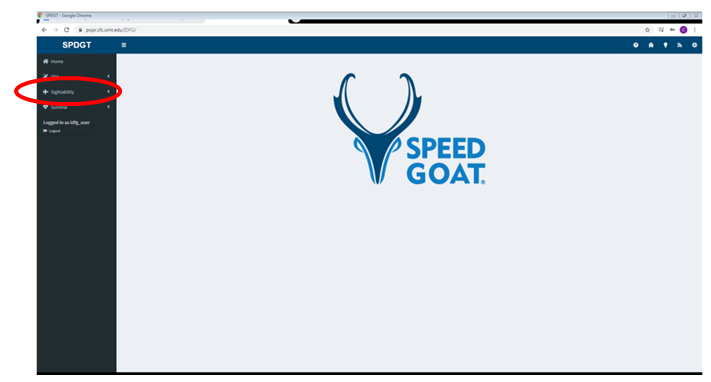
\includegraphics{./www/sight_01.PNG}

\begin{enumerate}
\def\labelenumi{\arabic{enumi}.}
\setcounter{enumi}{1}
\item
  Select the \textbf{Setup} page in the sidebar, then select the species and DAU you want to model. In this example we use mule deer and MD\_Smokey-Boise. Make sure to select the correct species and DAU before clicking the button to load sightability data.
\item
  Click the button labeled ``Get Survey Data'' to load the data for the species and DAU you selected.
\end{enumerate}

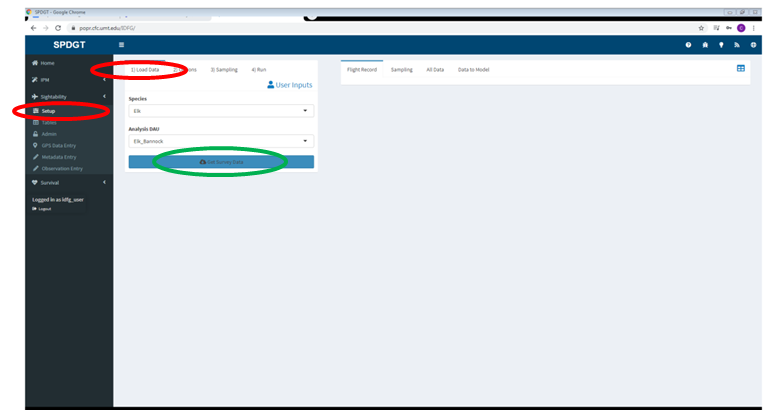
\includegraphics{./www/sight_02.PNG}

\begin{enumerate}
\def\labelenumi{\arabic{enumi}.}
\setcounter{enumi}{3}
\item
  Once the data is loaded you should see a dialog indicating that the process was successful. Click Dismiss. If you receive an error see the \protect\hyperlink{sight-errors}{errors} section.
\item
  Review the data in the panes to the right (see \protect\hyperlink{sight-load}{Loading Data} for details).
\end{enumerate}

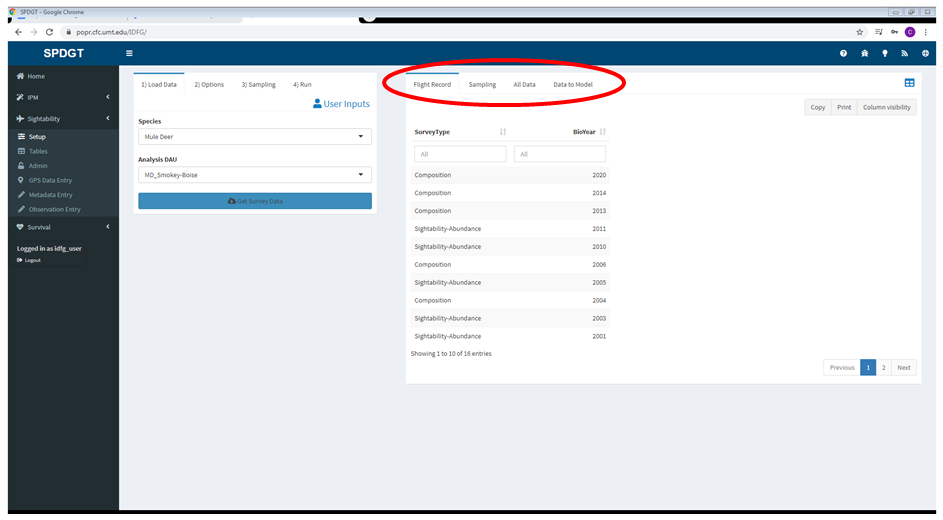
\includegraphics{./www/sight_03.PNG}

\begin{enumerate}
\def\labelenumi{\arabic{enumi}.}
\setcounter{enumi}{5}
\tightlist
\item
  Move on to the \protect\hyperlink{sight-options}{\textbf{Options}} tab in the \textbf{User Inputs} pane, and make the appropriate selections. In this example we run a model on 2020 composition data for mule deer, with area as the spatial focus of the analysis.
\end{enumerate}

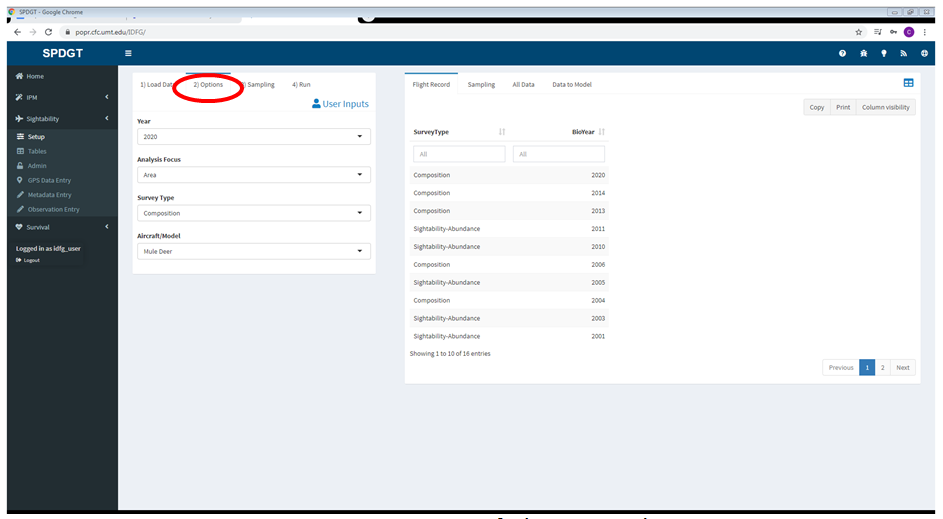
\includegraphics{./www/sight_04.PNG}

\begin{enumerate}
\def\labelenumi{\arabic{enumi}.}
\setcounter{enumi}{6}
\tightlist
\item
  Move on to the \protect\hyperlink{sight-options}{\textbf{Sampling}} tab and check that the data are accurate by selecting Sampling in the pane to the right. If the total population of subunits available in each stratum is incorrect you can fix it here.
\end{enumerate}

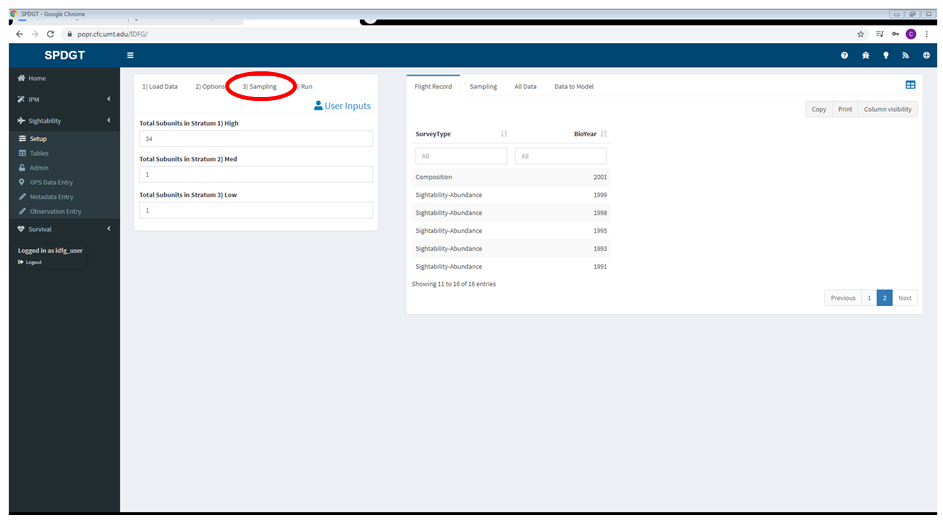
\includegraphics{./www/sight_05.PNG}

\begin{enumerate}
\def\labelenumi{\arabic{enumi}.}
\setcounter{enumi}{7}
\tightlist
\item
  Now that you've selected the appropriate settings and reviewed the input data, switch to the \textbf{Run} tab and click {Fit Model}.
\end{enumerate}

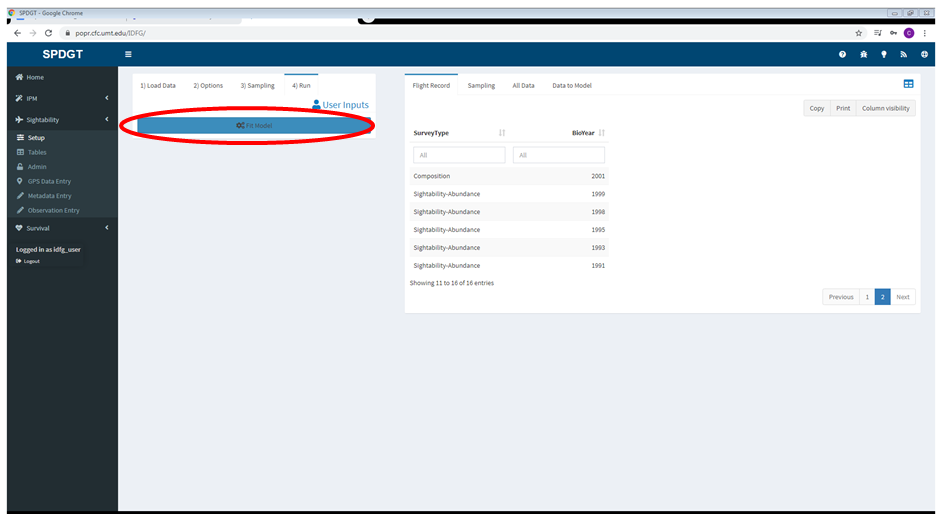
\includegraphics{./www/sight_06.PNG}

\begin{enumerate}
\def\labelenumi{\arabic{enumi}.}
\setcounter{enumi}{8}
\tightlist
\item
  Once model fitting is complete select the \textbf{Tables} page in the sidebar to view the output.
\end{enumerate}

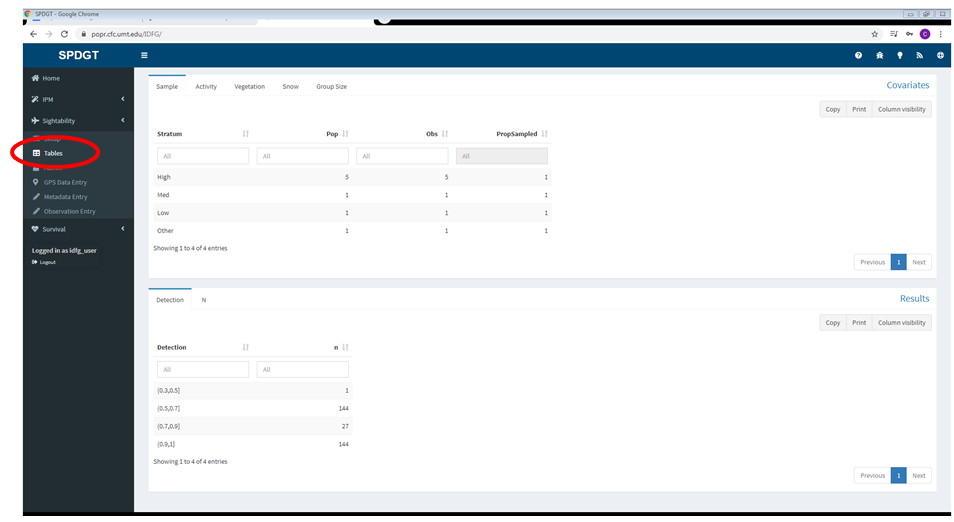
\includegraphics{./www/sight_07.PNG}

\begin{enumerate}
\def\labelenumi{\arabic{enumi}.}
\setcounter{enumi}{9}
\item
  The covariates section on the top half of the page summarizes the observations used in the model and how they fall into the various strata, activity categories, etc. See \protect\hyperlink{sight-output}{Model Output} for more details.
\item
  Select the \textbf{N} table on the bottom half of the screen to view abundance estimates.
\end{enumerate}

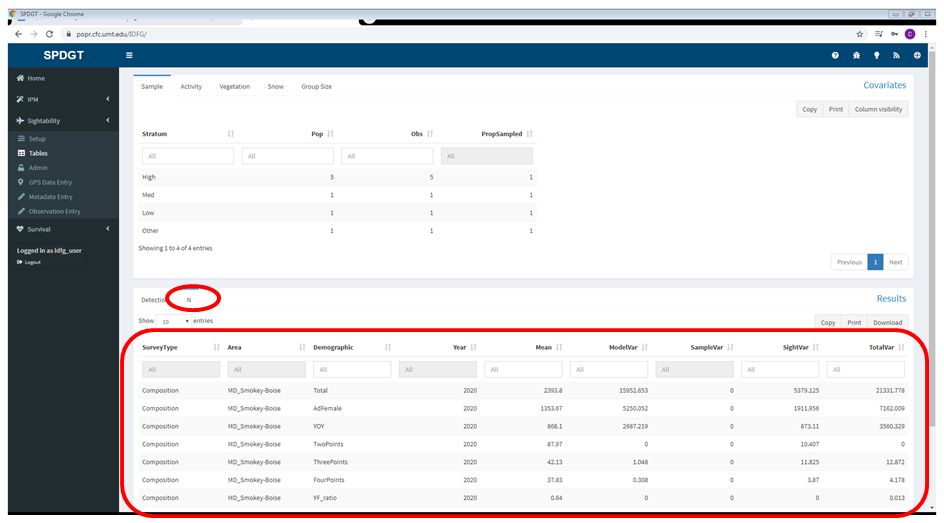
\includegraphics{./www/sight_08.PNG}

\begin{enumerate}
\def\labelenumi{\arabic{enumi}.}
\setcounter{enumi}{11}
\tightlist
\item
  Select the \textbf{Detection} table to view a summary of observations binned by probability of detection.
\end{enumerate}

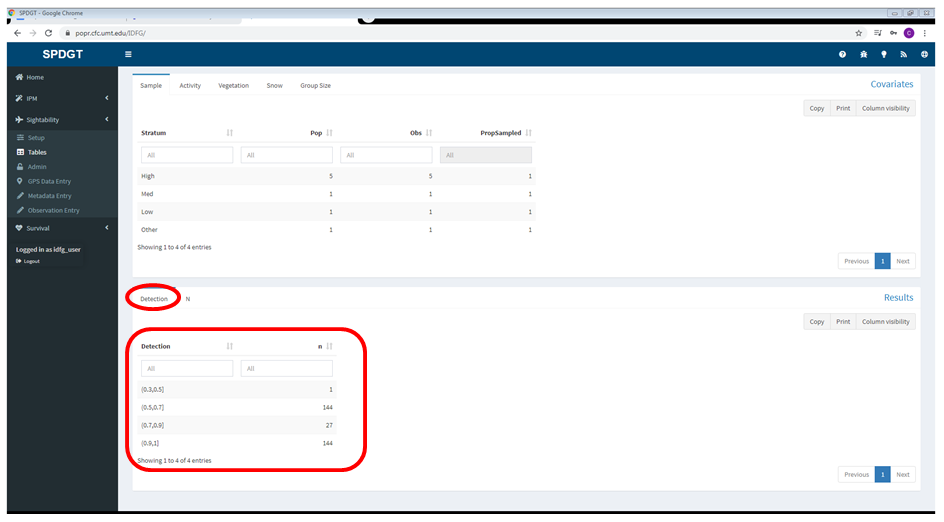
\includegraphics{./www/sight_09.PNG}

\begin{enumerate}
\def\labelenumi{\arabic{enumi}.}
\setcounter{enumi}{12}
\tightlist
\item
  If you're confident in the results and the settings used to run the model, you can add the sightability results to an \protect\hyperlink{gl-ipm-db}{IPM dataset} using the \textbf{Admin} tab in the sidebar. Be sure to read the \protect\hyperlink{sight-admin}{instructions} and understand the difference between the various IPM databases before using the admin tab.
\end{enumerate}

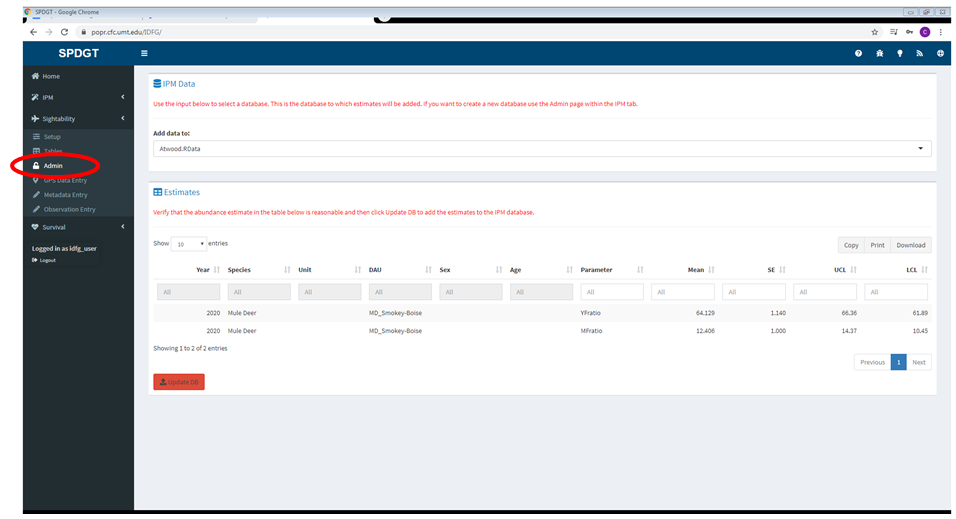
\includegraphics{./www/sight_15.PNG}

\hypertarget{surv}{%
\chapter{Survival}\label{surv}}

Estimating survival is a complicated process that reflects our inability to directly observe the quantity of interest. One way that we might start thinking about survival is by asking how many animals are alive at the end of some interval given how many started the interval. For example, we might collar 100 deer on the first of the month and then 30 days later we check on each animal and find that 98 deer are still alive. The expectation for survival then is 98/100 or 0.98. This simple expectation only works because the fate of ALL animals was known and every single individual was captured at the same time. This is not what happens in practice. When capture occurs animals are collared over a period of time that can span a few months. If we applied the same simple math as above we would not be very accurate because animals are exposed to risk for different amounts of time. For example, if we collar one deer on January 1 and another on March 1 and we want to know how many live until December we can't use division because one animal was available to die in several more months. Another wrinkle that often comes into play is collar failure. This essentially causes the animal to leave the sample and complicates estimation.

Sample size is a funny topic in survival modeling because very little information is contained in knowing the animal is alive, but we learn a lot when the animal dies. We basically need to observe lots of death. For example, the estimator above suggested 98/100, which is similar to the \href{https://en.wikipedia.org/wiki/Kaplan\%E2\%80\%93Meier_estimator\#:~:text=The\%20Kaplan\%E2\%80\%93Meier\%20estimator\%2C\%20also,amount\%20of\%20time\%20after\%20treatment.}{Kaplan-Meier} estimator (KM). Many agencies use the KM estimator because it is intuitive and relatively simple to implement. However, there are several problems with this approach and they appear at the extremes of sample size. One extreme is the case where 0 animals die, in this case the variance is undefined. Another extreme occurs in almost every study, as time marches on our sample size shrinks and eventually we may only have 10 or 20 animals marked. Let's say we have a study and only 10 animals are still on the air. If during the winter 4 of the animals die then we arrive at a survival estimate of 6/10 or 0.6. Is this correct? Not likely, not unless you really think that 40\% of the population perished. To make this point a little better say we only have 3 animals marked. What are the values of survival that we can estimate? Well, if 0 animals survive we can get 0, ⅓, ⅔ or 3/3. What if the true value of survival was something like 0.85? Turns out you can't even get that number from a sample size of three. The same is true of coin flips, if you flip a coin three times you can't get 0.5 the true probability of getting a heads.

With all of the complexities of survival estimation we generally have to write somewhat complicated models to get at the quantities of interest while protecting against bias. The models in PopR use a discrete-time known-fate approach to survival estimation. The models allow the user to estimate by age, sex, space and subset to different time intervals. We have written the models in this way to users to explore a variety of questions, share information among data rich and data poor areas and easily incorporate covariates. A nice example of the models in action is \href{https://wildlife.onlinelibrary.wiley.com/doi/full/10.1002/jwmg.21211}{Regional-scale models for predicting overwinter survival of mule deer} (Hurley et al.~2017). This paper will also give nice descriptions of the math and covariates used in predictions. One point to keep in mind is the idea of sharing information via random effects. The models and results in IPM database mule\_deer\_shared come from running a statewide model where information is shared among DAUs within a month. This means that the model can use all of the data from the state to figure out what an average, say, March survival should be and then further refine the estimate for any given DAU by also using the DAU specific data. I like to say that the model returns the statewide average when little to no data exist, but gives the opportunity to be different from the statewide average when sufficient data are present. The same DAU specific information can be extracted from these models. For example, if you want to know survival in March of 2019 in the Beaverhead DAU that information is available. The last feature of survival models that I will discuss are the multi-state models. These models allow the user to estimate not only survival, but the probability of death by harvest or death by some other cause. One equation to keep in mind here is Survival + Mortality = 1. This is always true and must be true. If 30\% of the population is harvested in a given year then the maximum value of survival is 0.7 if we assume that no animals died of any other cause. In fact, this equation is part of the reason why we care about abundance because the survival rate or harvest mortality rate can be applied to the abundance to determine the number of animals that died in a given year. Anyway, using the multi-state models the software will report Survival, Harvest Mortality and Other Mortality. Remember that if you are conditioned to seeing survival with harvest removed then survival is equal to 1 - other mortality. For example, I expect adult female mule deer survival to be about 0.85 in the absence of harvest and I might get that value if I censor harvest in the known fate model. However, because survival + harvest mortality + other mortality = 1 the survival from the multi-state model will be lower. If we rearrange the above equation to solve for survival + harvest than we will probably get a number like 0.85 from 1 - other mortality = survival + harvest mortality, which is essentially the probability of surviving non-harvest causes of death.

\hypertarget{surv-model}{%
\section{Running a Survival Model}\label{surv-model}}

\hypertarget{surv-load}{%
\subsection{Loading Data}\label{surv-load}}

To run a survival model select \textbf{Survival} in the sidebar then click \textbf{Setup}. Select a species and \protect\hyperlink{gl-dau}{DAU} on the Overview tab and click the {Download Data} button to download data from the \protect\hyperlink{gl-samm}{IDFG database}. Once the download is complete a dialog will confirm that the data has been downloaded and alert you to any errors present in the data (see the \protect\hyperlink{surv-errors}{errors} section). Data will only be read for the species and DAU selected, so if you switch either selection later you'll have to repeat the process.

Once the data is downloaded you can review it in various formats in the pane to the right. Data is pulled from \protect\hyperlink{gl-samm}{SAMM}, so if you find individuals that plot out in the wrong area or DAU, you'll need to fix them there.

\begin{itemize}
\tightlist
\item
  Captures: Shows a map of the capture locations of all the individuals used in the analysis. The table on the left shows any IDs that have bad or missing capture location information.
\item
  Mortalities: Shows a map of the mortality locations for the DAU. The table on the left shows any IDs that have bad or missing mortality location information.
\item
  Collared Animals: Shows a barplot of the number of collared individuals throughout the analysis years. You can hover over each bar with your mouse and at the top of the graph, it will show you the status of collared individuals by month. Categories include missing, other mortality, harvested, and alive.
\item
  Raw Data Summary: Shows a summary of the raw data available to be for the selected DAU.
\end{itemize}

All the data available for the selected DAU can be viewed using the Captures, Monitoring, Mortalities, Encounter Histories, and Raw Data tabs in the bottom table. The Captures and Mortalities tables show information for \emph{all} individuals, even if capture/mortality information is unavailable. You can sort using the arrows next to the headings and filter by entering names/values into the boxes under the headings.

You can also view the data loaded from SADD on the \textbf{Individuals} page, where you can view raw data, encounter histories, captures, and mortality records. You can also filter to a specific animal, which can be helpful in tracking down \protect\hyperlink{surv-errors}{errors}.

\hypertarget{surv-options}{%
\subsection{Model Options}\label{surv-options}}

After loading survival data for a particular species and DAU move on to the Subset tab to specify the parameters for your model. Select a sex (default is all) and \protect\hyperlink{gl-age-classes}{age class} (default is adult) to model, then select the range of years to include in the analysis (default includes all data available).

Move on to the Structure tab and use the inputs to define the model that will be run on your data. First select a \protect\hyperlink{gl-known-fate}{known fate} (simple survival estimation) or \protect\hyperlink{gl-multi-state}{multi-state} (estimate mortality rates by cause - currently unavailable) model. If you're running a multi-state model use the Censor Fate input to exclude a particular source of mortality from the analysis. For example, if harvest is selected the estimated survival will answer the question ``What would survival be in the absence of harvest?'' Finally define how survival is allowed to vary with sex, time, and space. You must select more than 5 years for analysis to model survival as varying through time, and modeling survival as spatially varying is only available for statewide models.

If you plan on adding your results to an \protect\hyperlink{gl-ipm-db}{IPM dataset} you should use the default settings:

\begin{itemize}
\tightlist
\item
  Sex: All
\item
  Age: One at a time, A then J
\item
  Analysis Years: 2000-Current Year
\item
  Model Type: Known Fate
\item
  Covariates: None
\item
  Censor Fate(s): Harvest
\item
  Model sexes as: Different
\item
  Model time as: Monthly
\item
  Model space as: Varying
\item
  Thinning Rate: 1
\item
  Burnin Length: 35,000
\item
  MCMC Iterations: 25,000
\end{itemize}

When you've loaded your data, selected the appropriate options, and defined your model structure, move on to the Run tab, specify your \protect\hyperlink{gl-mcmc}{MCMC settings}, and click {Fit Model} to run the model. If no errors are encountered dismiss the dialog and click \textbf{Tables} in the sidebar to view your results. If the model fails to run check the \protect\hyperlink{surv-errors}{errors} section.

\hypertarget{surv-output}{%
\subsection{Model Output}\label{surv-output}}

Results are viewed under the \textbf{Tables} subheading on the left under \textbf{Survival}. Estimates can be viewed by year or by month. Mean estimates are accompanied by the standard deviation as well as the lower and upper confidence intervals. You can copy, print, or download the data using the buttons at the top right of the table. You can also sort and filter using the boxes below the column headings.

\hypertarget{surv-admin}{%
\subsection{Adding Results to IPM}\label{surv-admin}}

Use the \textbf{Admin} page to add the results of your survival model to the input data for the IPM. Only add the results to an \protect\hyperlink{gl-ipm-db}{IPM dataset} if you're sure you used the correct settings and data. If there is already survival data in the IPM data file you select for the same species, year, and unit, that data will be overwritten with the results of your current model.

Select the \protect\hyperlink{gl-ipm-db}{IPM dataset} to which you want to add your estimates, and verify that the estimates themselves look reasonable, then click {Update DB} to add the estimates to the database file. DO NOT add results to the IPM database if you didn't use the default settings outlined in the \protect\hypertarget{surv-options}{}{Model Options} section.

\hypertarget{surv-errors}{%
\subsection{Errors}\label{surv-errors}}

\hypertarget{reporting-errors-1}{%
\subparagraph*{Reporting errors}\label{reporting-errors-1}}
\addcontentsline{toc}{subparagraph}{Reporting errors}

This section of the documentation is a work in progress. We need your feedback to identify and document the errors users commonly experience running models with PopR - you can help us by sending an email to \href{mailto:eric.newkirk@speedgoat.io?cc=josh.nowak@speedgoat.io\&subject=PopR\%20Error}{eric.newkirk@speedgoat.io} any time you experience an error on the site. Please include as much information as you can about your settings, data, and the error message you received, including screenshots if possible. Thanks!

\hypertarget{surv-ex}{%
\section{Step-By-Step Survival Model Example}\label{surv-ex}}

This example shows how to run a survival model for mule deer in the Smokey-Boise DAU step by step, including screenshots of the website.

\begin{enumerate}
\def\labelenumi{\arabic{enumi}.}
\tightlist
\item
  Start by clicking \textbf{Survival} in the sidebar.
\end{enumerate}

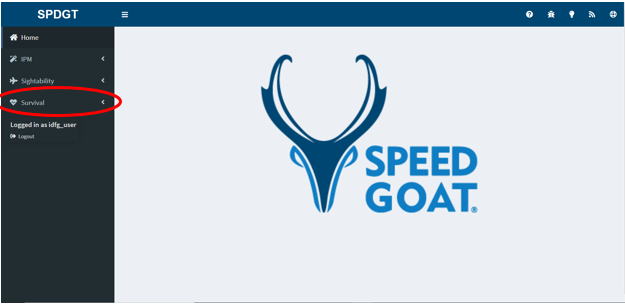
\includegraphics{./www/surv_01.PNG}

\begin{enumerate}
\def\labelenumi{\arabic{enumi}.}
\setcounter{enumi}{1}
\item
  Select the \textbf{Setup} page in the sidebar, then select the species and DAU you want to model. In this example we use mule deer and MD\_Smoky-Boise. Make sure to select the correct species and DAU before clicking the button to load sightability data.
\item
  Click the button labeled ``Download Data'' to load the data for the species and DAU you selected.
\end{enumerate}

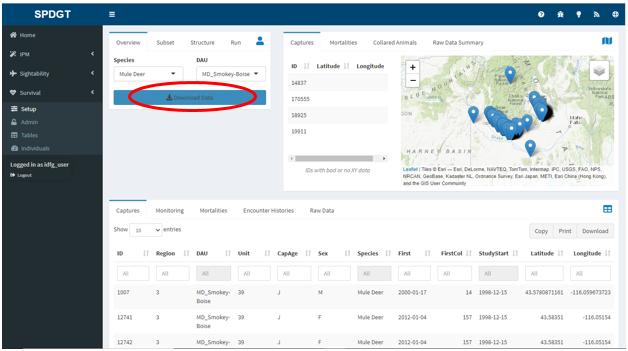
\includegraphics{./www/surv_02.PNG}

\begin{enumerate}
\def\labelenumi{\arabic{enumi}.}
\setcounter{enumi}{3}
\item
  Once the data is loaded you should see a dialog indicating that the process was successful. Click Dismiss. If you receive an error see the \protect\hyperlink{surv-errors}{errors} section.
\item
  Review the data in the panes to the right and tables at the bottom (see \protect\hyperlink{surv-load}{Loading Data} for details).
\end{enumerate}

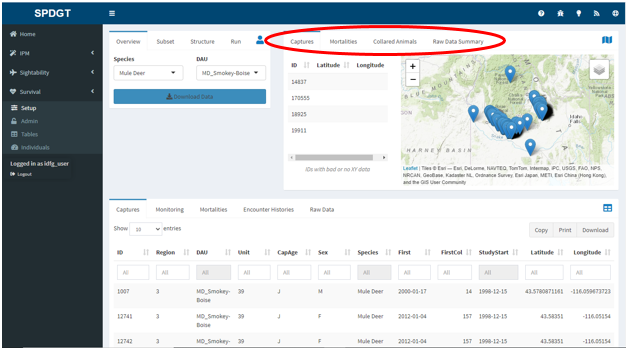
\includegraphics{./www/surv_04.PNG}

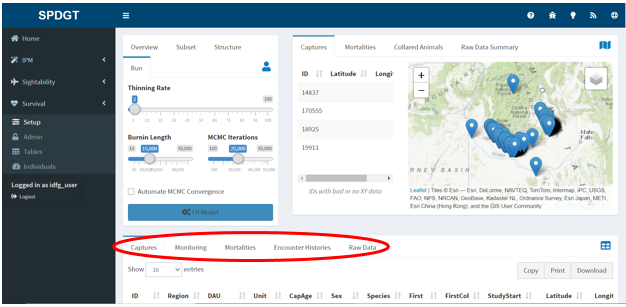
\includegraphics{./www/surv_05.PNG}

\begin{enumerate}
\def\labelenumi{\arabic{enumi}.}
\setcounter{enumi}{5}
\tightlist
\item
  Move on to the \protect\hyperlink{surv-options}{\textbf{Subset}} tab in the \textbf{User Inputs} pane, and make the appropriate selections. In this example we ran a model for adults of both sexes using data from 2000 to 2020.
\end{enumerate}

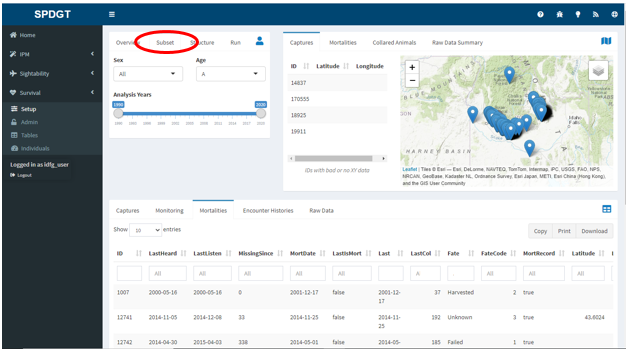
\includegraphics{./www/surv_06.PNG}

\begin{enumerate}
\def\labelenumi{\arabic{enumi}.}
\setcounter{enumi}{6}
\tightlist
\item
  Move on to the \protect\hyperlink{surv-options}{\textbf{Structure}} tab and define the model you want to run. Here we use a \protect\hyperlink{gl-known-fate}{known fate} model where survival does not vary with sex, space, or time.
\end{enumerate}

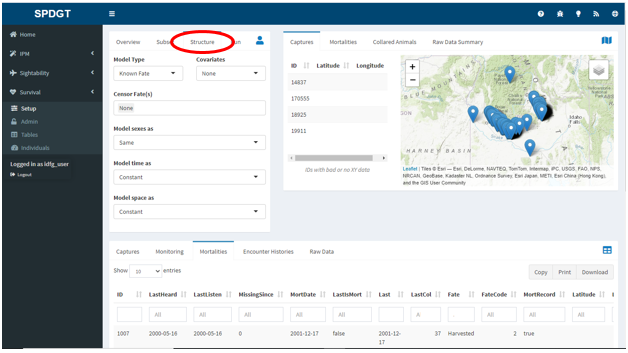
\includegraphics{./www/surv_07.PNG}

\begin{enumerate}
\def\labelenumi{\arabic{enumi}.}
\setcounter{enumi}{7}
\tightlist
\item
  Now that you've selected the appropriate settings and reviewed the input data, switch to the \textbf{Run} tab and click {Fit Model}.
\end{enumerate}

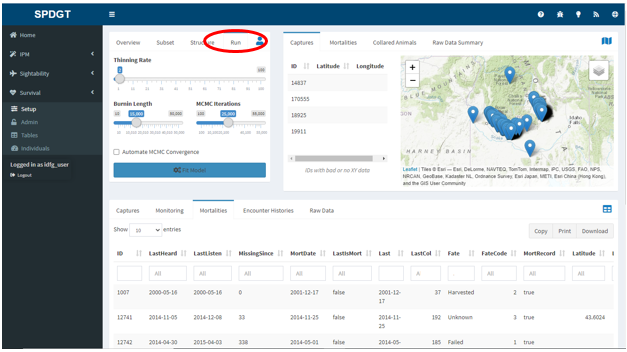
\includegraphics{./www/surv_08.PNG}

\begin{enumerate}
\def\labelenumi{\arabic{enumi}.}
\setcounter{enumi}{8}
\tightlist
\item
  Once model fitting is complete select the \textbf{Tables} page in the sidebar to view the output.
\end{enumerate}

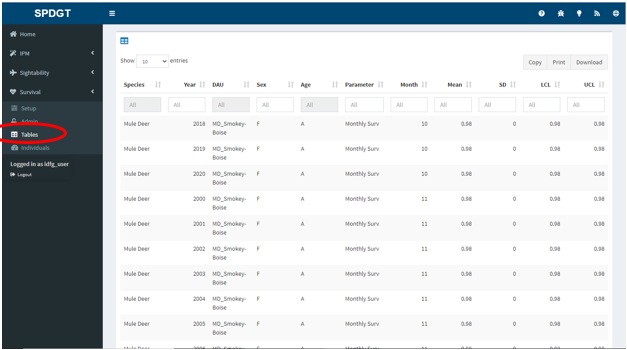
\includegraphics{./www/surv_10.PNG}

\begin{enumerate}
\def\labelenumi{\arabic{enumi}.}
\setcounter{enumi}{9}
\tightlist
\item
  If you're confident in the results and the settings used to run the model, you can add the survival results to an \protect\hyperlink{gl-ipm-db}{IPM dataset} using the \textbf{Admin} tab in the sidebar. Be sure to read the \protect\hyperlink{surv-admin}{instructions} and understand the difference between the various IPM databases before using the admin tab.
\end{enumerate}

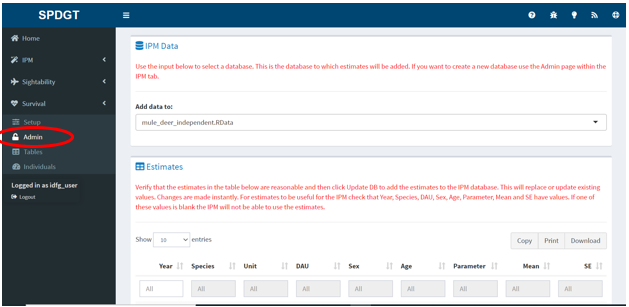
\includegraphics{./www/surv_12.PNG}

\hypertarget{ipm}{%
\chapter{IPM}\label{ipm}}

PopR allows you to combine data from various sources to model wildlife populations using an integrated population model (IPM), leading to more robust and defensible estimates. First the data from each source are modeled independently to estimate individual population parameters, such as sex ratio and survival. Then these results are combined in the IPM to find the best fit for all of the available data.

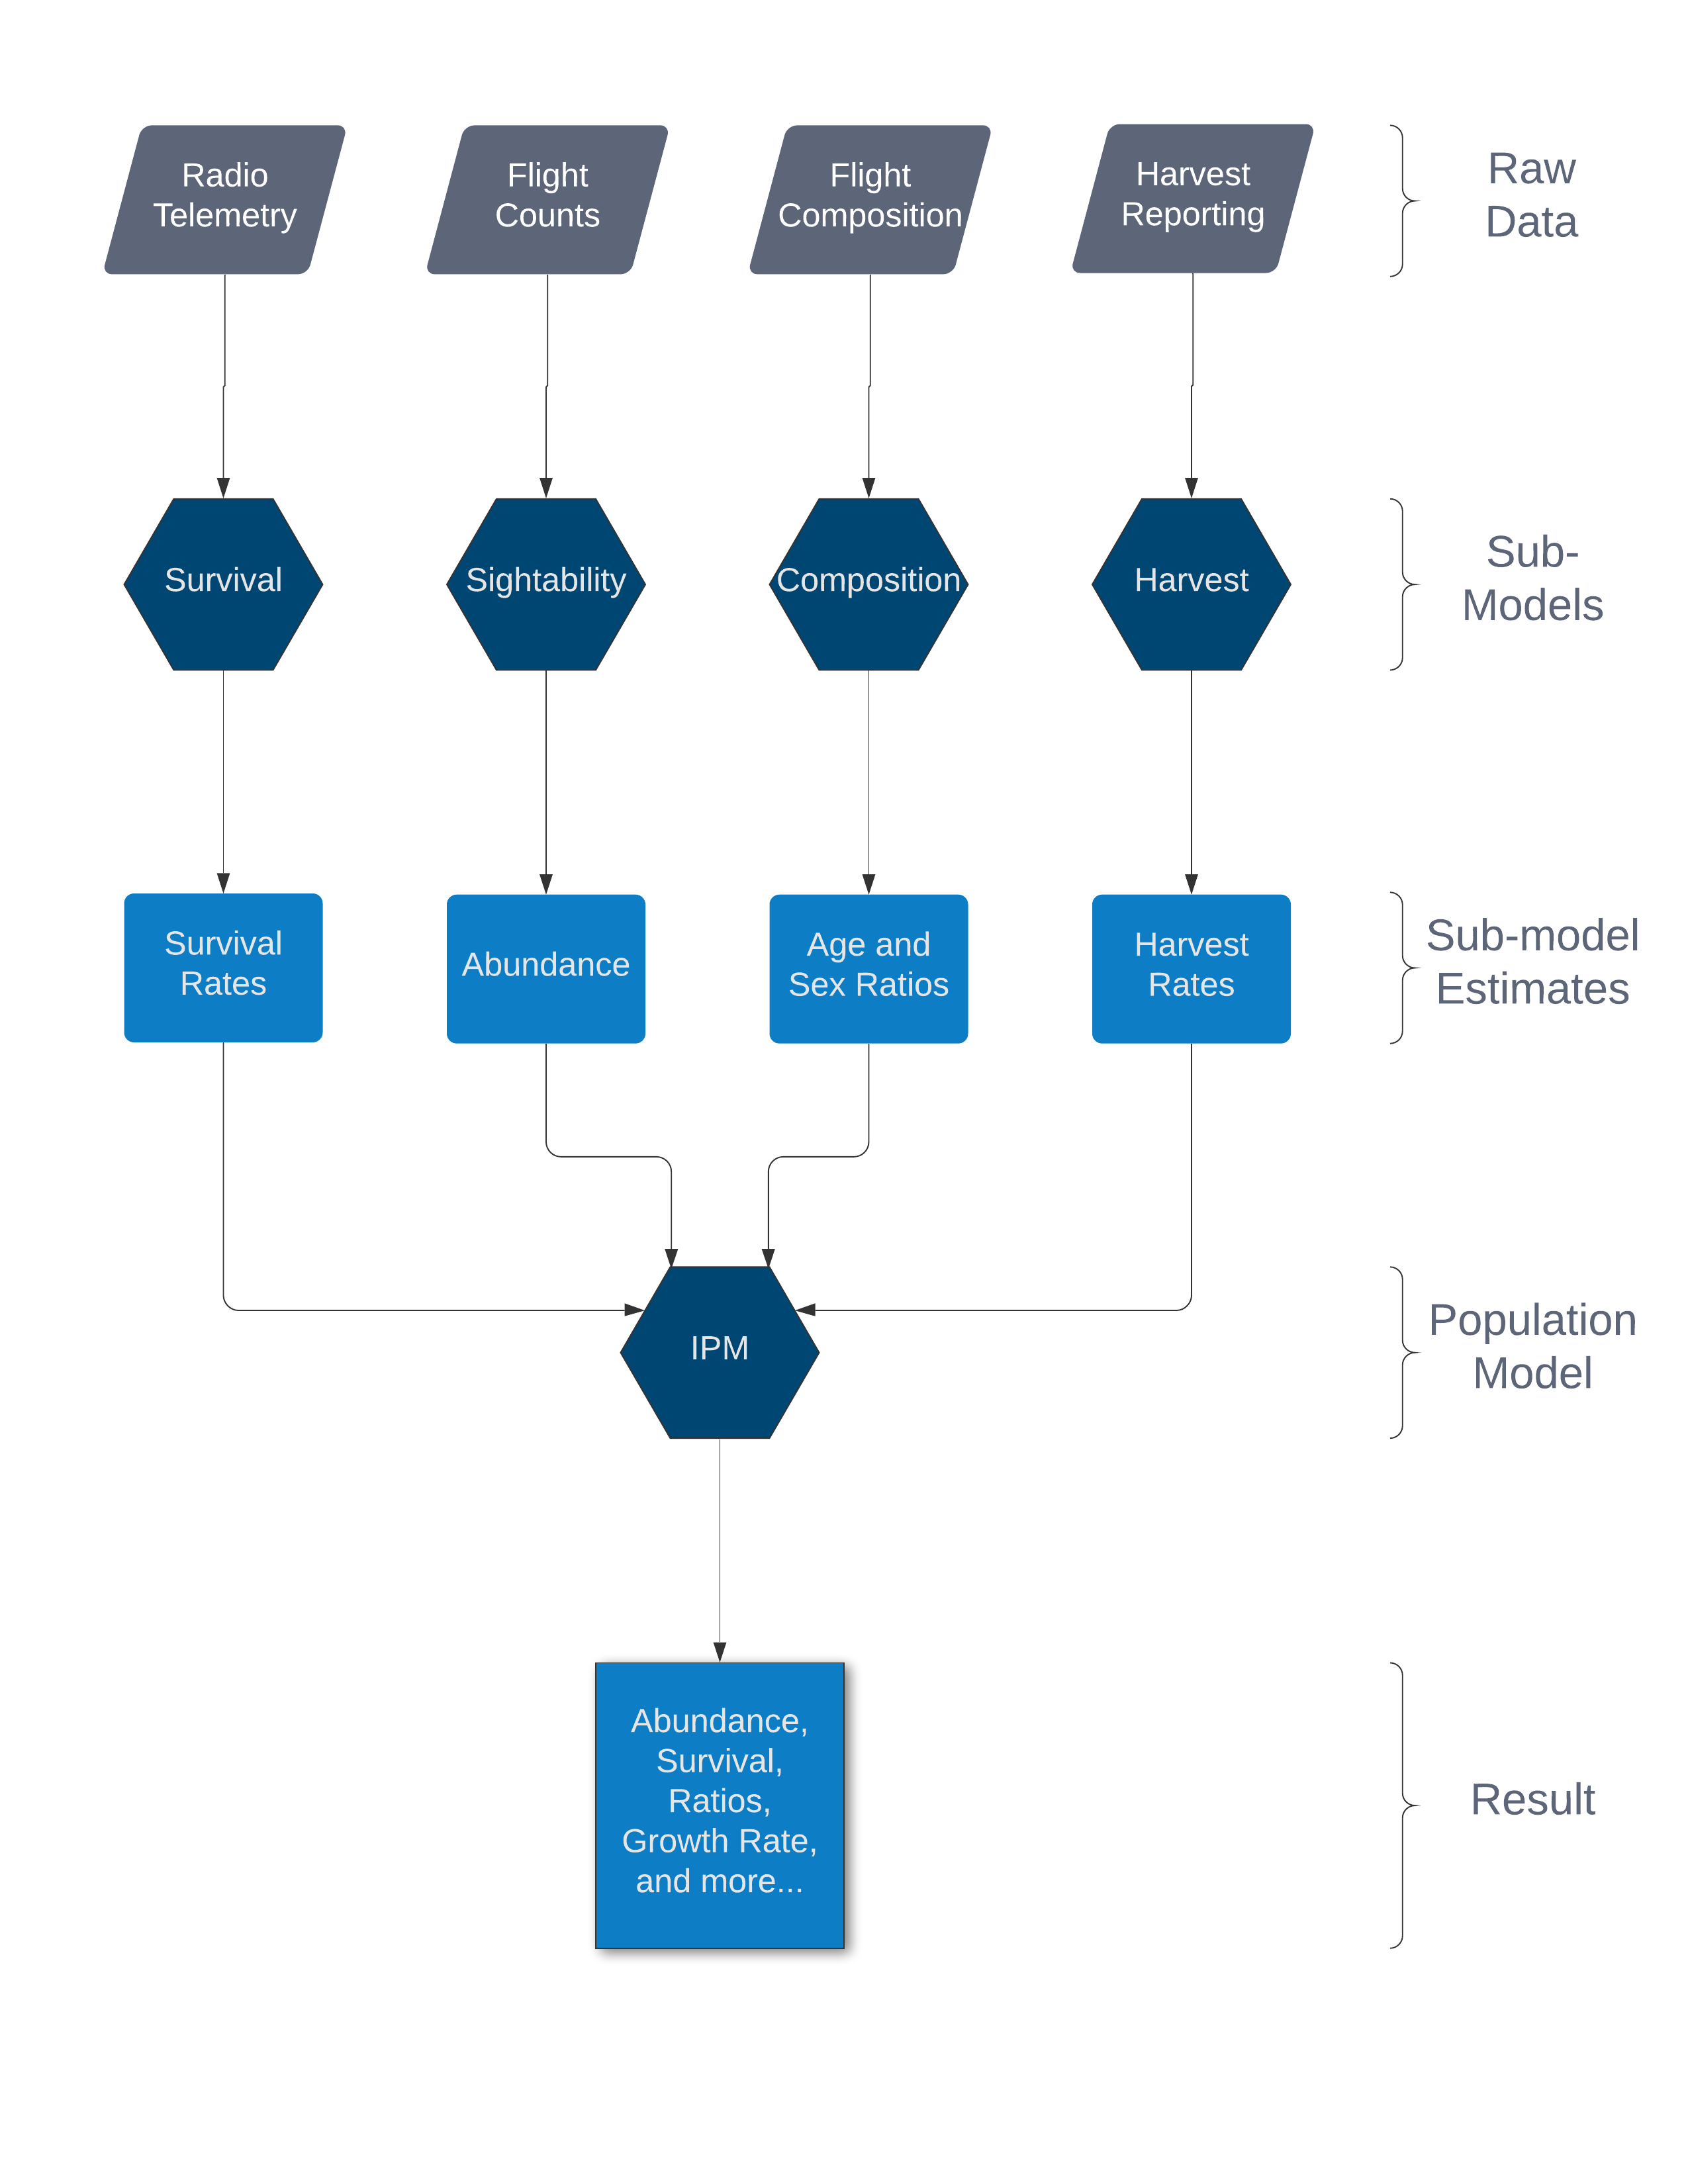
\includegraphics{./www/ipm_flowchart.PNG}

\hypertarget{ipm-model}{%
\section{Running the IPM}\label{ipm-model}}

\hypertarget{ipm-load}{%
\subsection{Loading Data}\label{ipm-load}}

To run an integrated population model select \textbf{IPM} in the sidebar then click \textbf{Setup}. Running an IPM requires 2 types of data: population estimates from an \protect\hyperlink{gl-ipm-db}{IPM database} and harvest data from the IDFG database. Start by selecting a species and DAU on the Overview tab, then select the IPM database you want to use and choose how the model incorporates \protect\hyperlink{gl-ipm-weather}{future weather}. At this point you can review the population estimates from previous models in the plots to the right and the tables along the bottom, but notice that there is no data available in the Harvest tabs. To fix that click the {Fetch Harvest Data} button to download the appropriate data from the IDFG database. Once the download is complete a dialog will confirm that the data has been downloaded and alert you to any errors present in the data (see the \protect\hyperlink{ipm-errors}{errors} section). Now you can review the harvest data in the plots and tables in addition to the population estimates. Data will only be read for the species and DAU selected, so if you switch either selection later you'll have to download harvest data again.

Once you've loaded estimates from the IPM database and downloaded harvest data from SADD you can review everything in the plots to the right and tables below. All data available to the IPM for analysis is shown in these panes. If you cannot find data that should be used by the IPM for analysis in either of these areas then that data has not been made available to the model. This may indicate that the missing data needs to be passed to the IPM via the \protect\hyperlink{sight}{sightability} or \protect\hyperlink{surv}{survival} tabs.

\hypertarget{ipm-options}{%
\subsection{Model Options}\label{ipm-options}}

After loading data for a particular species and DAU move on to the Structure tab and use the inputs to define the model that will be run on your data. Use the inputs to define whether the model uses population reconstruction and whether reproduction and survival vary by year or remain constant. If you want to run the IPM with default settings for the current species click the {Default Structure} button below the inputs to load the default settings listed here:

\begin{itemize}
\tightlist
\item
  Use Population Reconstruction: No
\item
  Reproduction: Time Varying
\item
  Juvenile Survival: Time Varying
\item
  Subadult Survival: Constant (elk only)
\item
  Adult Survival: Constant
\end{itemize}

If the IPM doesn't run or produces poor results with these defaults you can try adjusting the settings to better match the available data, but keep in mind that at least one of the variables must be constant (rather than time varying) for the IPM to work.

The harvest tab allows you to predict future harvest rates and incorporate those predictions into the IPM. First use the slider at the top to select the range of years for which you want to estimate abundance. If your selected range extends beyond the available harvest data use the additional sliders to specify how many animals you expect to be harvested by sex. You can use the \textbf{Options} button to set the sliders to the min, mean, median, or max from the existing harvest data, or to use the most recent data available (last). You can also click {Reset} to return to the default (mean) values. Be sure to click on the Harvest tab to the right to preview how your settings will be passed into the IPM.

When you've loaded your data, defined your model structure, and provided future harvest estimates (if needed), move on to the Run tab, specify your \protect\hyperlink{gl-mcmc}{MCMC settings}, and click {Fit Model} to run the IPM. If no errors are encountered dismiss the dialog and click \textbf{Tables} in the sidebar to view your results. If the model fails to run check the \protect\hyperlink{surv-errors}{errors} section.

\hypertarget{ipm-output}{%
\subsection{Model Output}\label{ipm-output}}

Results are viewed under the \textbf{Plots} and \textbf{Tables} subheadings on the left under \textbf{IPM}. On the tables tab you can view all of the abundance estimates by year, \protect\hyperlink{gl-age-classes}{age class}, and sex. The mean estimate, standard deviation, and confidence intervals are reported, along with the \protect\hyperlink{gl-rhat}{BGR diagnostic} in the Rhat column. Values greater than 1.1 in this column indicate poor model fit, in which case you may want to adjust the \protect\hyperlink{ipm-options}{model structure} or MCMC settings. Values at or near 1, on the other hand, indicate the model fit the data well.

The \textbf{Plots} page shows the estimates plotted over time. Plots are grouped into 4 categories based on the population parameter displayed:

\begin{itemize}
\tightlist
\item
  Abundance

  \begin{itemize}
  \tightlist
  \item
    Total abundance
  \item
    Female abundance by age class
  \item
    Male abundance by age class
  \end{itemize}
\item
  Ratios

  \begin{itemize}
  \tightlist
  \item
    Age ratio (young per adult female)
  \item
    Sex ratio (adult male per adult female)
  \end{itemize}
\item
  Survival

  \begin{itemize}
  \tightlist
  \item
    Female survival by age class
  \item
    Male survival by age class
  \end{itemize}
\item
  Misc

  \begin{itemize}
  \tightlist
  \item
    Growth Rate (λ)
  \item
    Maximum Sustained Yield (MSY - shows how growth rate, recruitment, and juvenile survival vary with total abundance)
  \item
    Harvest Rate by sex
  \item
    Harvest by sex
  \end{itemize}
\end{itemize}

All plots have tools along the right side which allow the user to zoom in on different sections of the graph, hover over specific points to get detailed information, and save/download as an image file.

To generate a report click on \textbf{Build Report} in the sidebar, then click {Download}. When the download is finished click on the saved html file to open it. The report combines information about your settings, input data, and results in a single file. Especially important in the report is the Diagnostics section, which explains how well the model performed and provides guidance on any changes that might improve your results.

\hypertarget{ipm-errors}{%
\subsection{Errors}\label{ipm-errors}}

\hypertarget{reporting-errors-2}{%
\subparagraph*{Reporting errors}\label{reporting-errors-2}}
\addcontentsline{toc}{subparagraph}{Reporting errors}

This section of the documentation is a work in progress. We need your feedback to identify and document the errors users commonly experience running models with PopR - you can help us by sending an email to \href{mailto:eric.newkirk@speedgoat.io?cc=josh.nowak@speedgoat.io\&subject=PopR\%20Error}{eric.newkirk@speedgoat.io} any time you experience an error on the site. Please include as much information as you can about your settings, data, and the error message you received, including screenshots if possible. Thanks!

\hypertarget{ipm-ex}{%
\section{Step-By-Step IPM Example}\label{ipm-ex}}

This example shows how to run the IPM for mule deer in the Bannock DAU step by step, including screenshots of the website.

\begin{enumerate}
\def\labelenumi{\arabic{enumi}.}
\tightlist
\item
  Start by clicking \textbf{IPM} in the sidebar.
\end{enumerate}

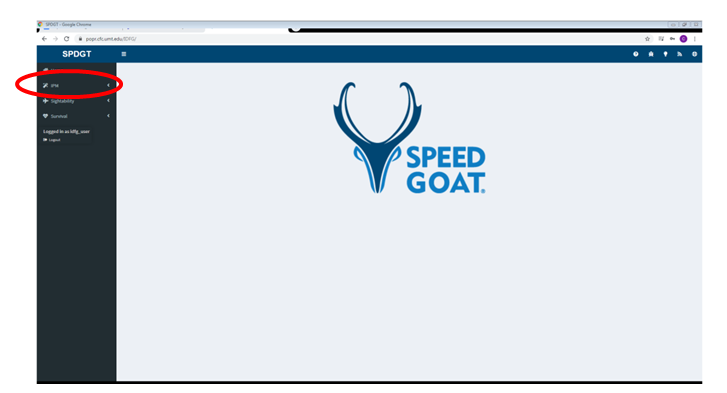
\includegraphics{./www/ipm_01.PNG}

\begin{enumerate}
\def\labelenumi{\arabic{enumi}.}
\setcounter{enumi}{1}
\item
  Select the \textbf{Setup} page in the sidebar, then select the species and DAU you want to model. Select the \protect\hyperlink{gl-ipm-db}{IPM database} containing the estimates you want to use, and choose an option for incorporating {[}weather covariates{]}(\#gl-ipm-weather\}.In this example we use mule deer and Bannock. Make sure to select the correct species and DAU before clicking the button to load harvest data.
\item
  Click the button labeled ``Fetch Harvest Data'' to load the data for the species and DAU you selected.
\end{enumerate}

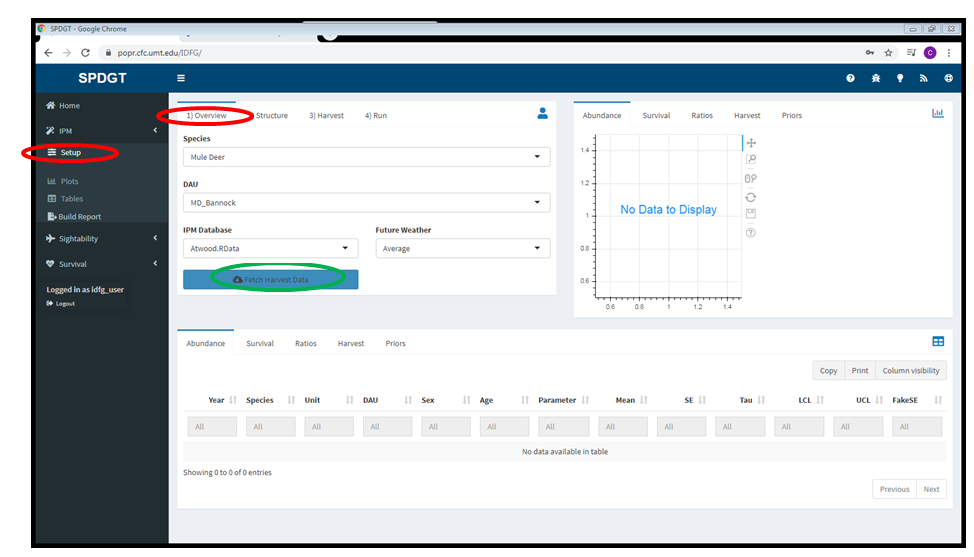
\includegraphics{./www/ipm_02.PNG}

\begin{enumerate}
\def\labelenumi{\arabic{enumi}.}
\setcounter{enumi}{3}
\item
  Once the data is loaded you should see a dialog indicating that the process was successful. Click Dismiss. If you receive an error see the \protect\hyperlink{ipm-errors}{errors} section.
\item
  Review the data in the panes to the right and tables at the bottom (see \protect\hyperlink{ipm-load}{Loading Data} for details).
\end{enumerate}

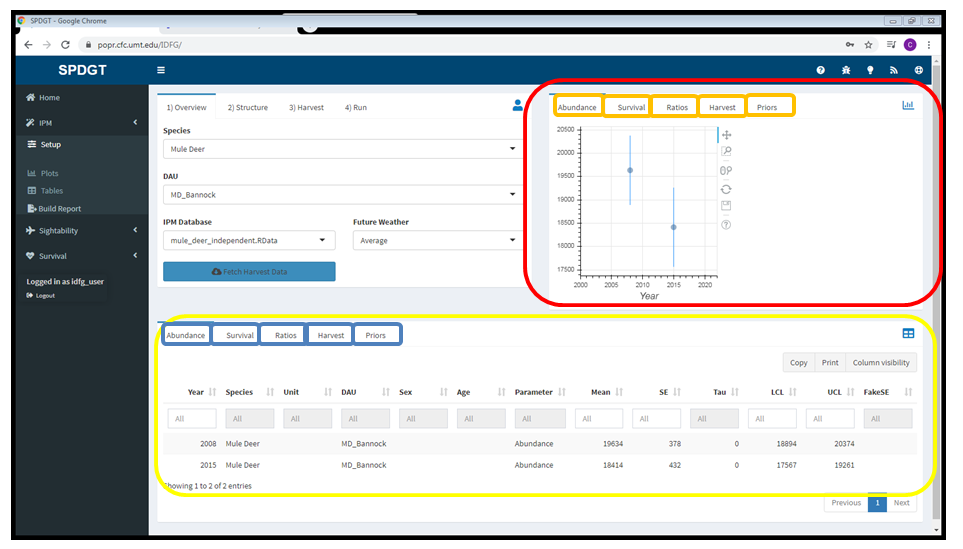
\includegraphics{./www/ipm_03.PNG}

\begin{enumerate}
\def\labelenumi{\arabic{enumi}.}
\setcounter{enumi}{5}
\tightlist
\item
  In this example, the abundance data that will be used by the IPM was collected in the Bannock DAU in 2008 and 2015 shown in the graph in the upper right (red rectangle) and in the table at the bottom of the page (yellow rectangle).
\end{enumerate}

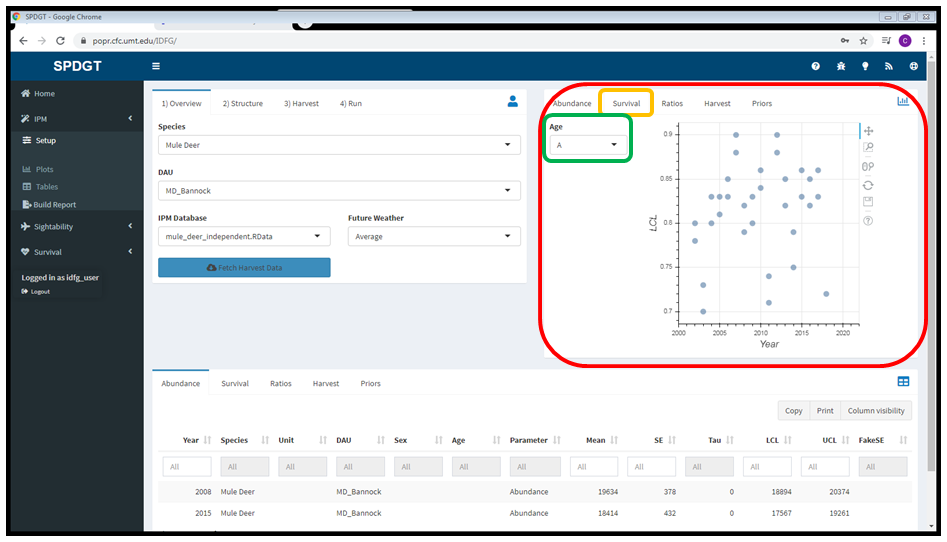
\includegraphics{./www/ipm_04.PNG}

\begin{enumerate}
\def\labelenumi{\arabic{enumi}.}
\setcounter{enumi}{6}
\tightlist
\item
  Move on to the \protect\hyperlink{ipm-options}{\textbf{Structure}} tab and click the button to apply the default settings. Your settings should match those in the screenshot below.
\end{enumerate}

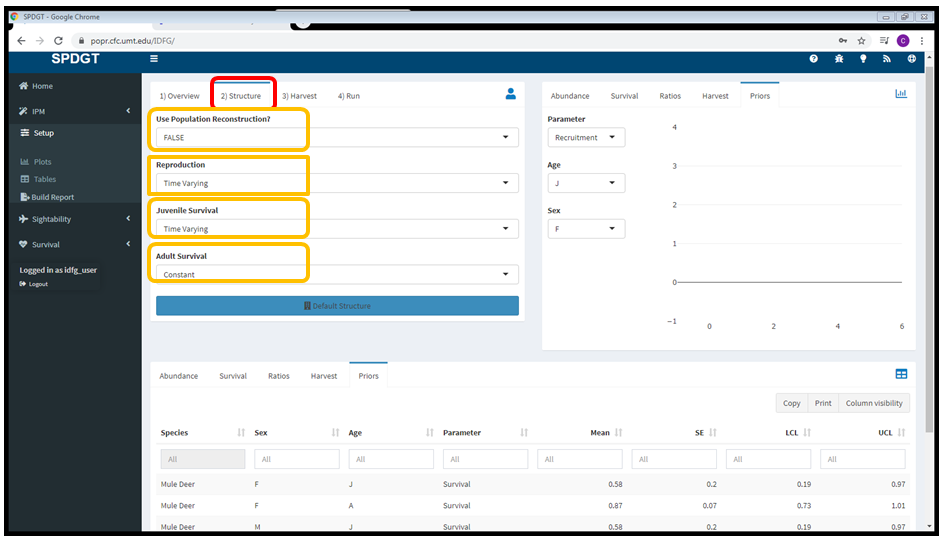
\includegraphics{./www/ipm_06.PNG}

\begin{enumerate}
\def\labelenumi{\arabic{enumi}.}
\setcounter{enumi}{7}
\tightlist
\item
  Continue to the \protect\hyperlink{ipm-options}{\textbf{Harvest}} tab to review the settings there. The defaults were used for this example, so there's no need to change anything.
\end{enumerate}

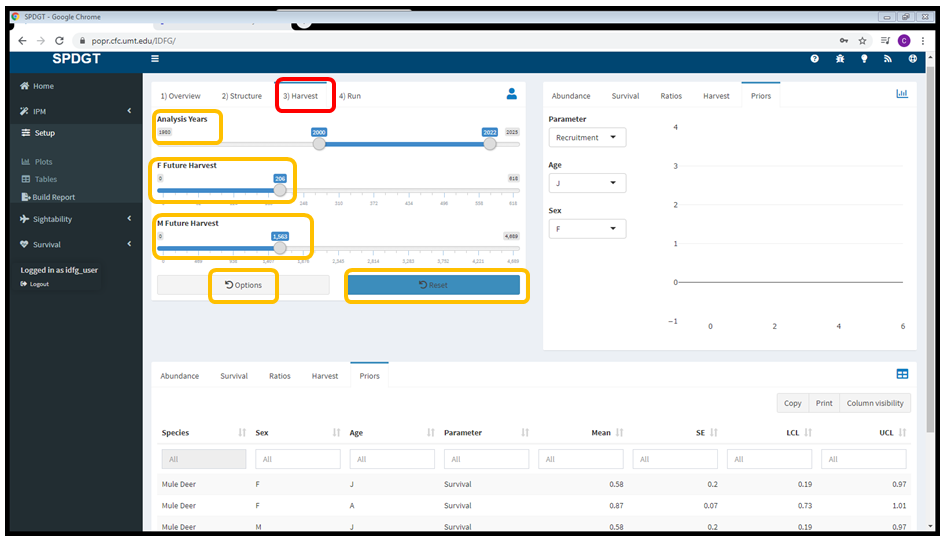
\includegraphics{./www/ipm_07.PNG}

\begin{enumerate}
\def\labelenumi{\arabic{enumi}.}
\setcounter{enumi}{8}
\tightlist
\item
  Now that you've selected the appropriate settings and reviewed the input data, switch to the \textbf{Run} tab. Change the burn in slider to 10,500, change the number of iterations to 41,000, and click {Fit Model}.
\end{enumerate}

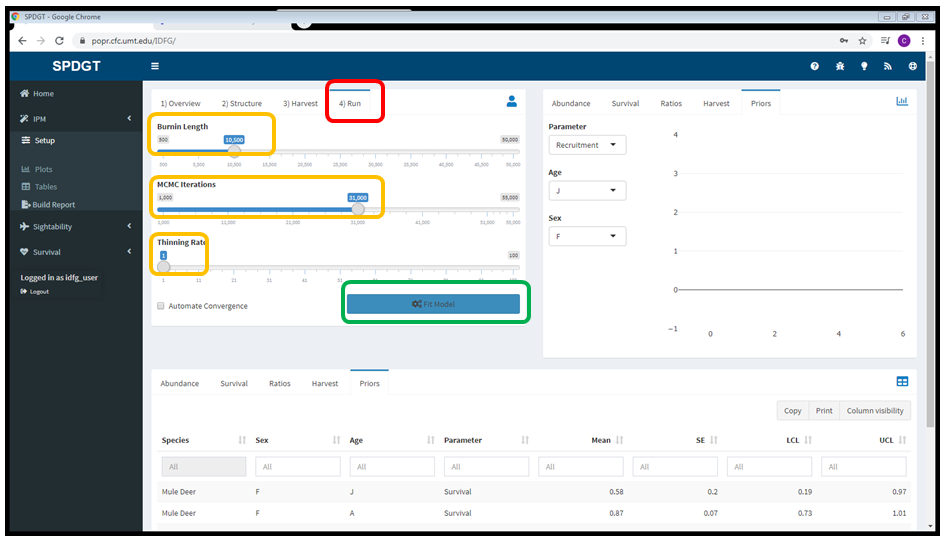
\includegraphics{./www/ipm_08.PNG}

\begin{enumerate}
\def\labelenumi{\arabic{enumi}.}
\setcounter{enumi}{9}
\tightlist
\item
  Once model fitting is complete select the \textbf{Plots} page in the sidebar to view the output.
\end{enumerate}

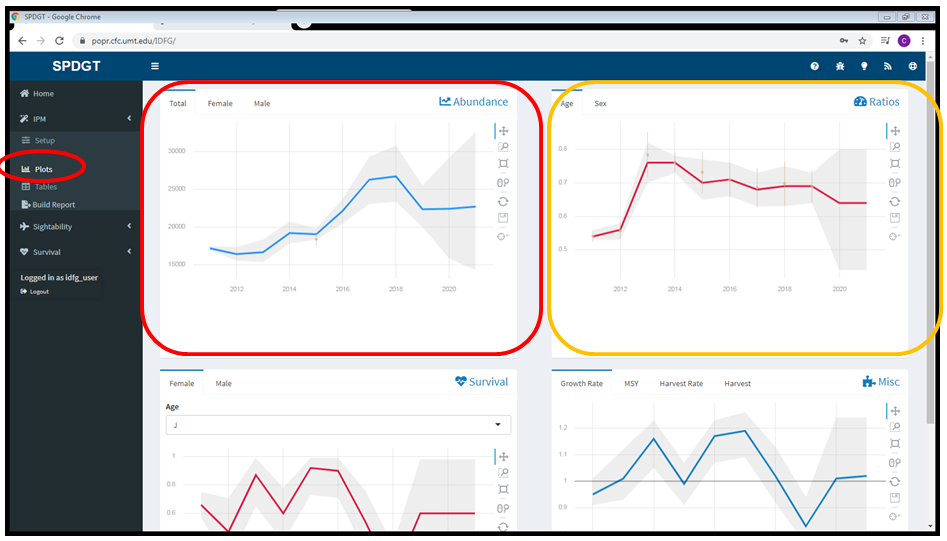
\includegraphics{./www/ipm_09.PNG}

\begin{enumerate}
\def\labelenumi{\arabic{enumi}.}
\setcounter{enumi}{10}
\tightlist
\item
  Check the \textbf{Tables} page as well to see how the model performed. Note the Rhat values (\textgreater{} 1.1) that appear in red, indicating the model may not have converged.
\end{enumerate}

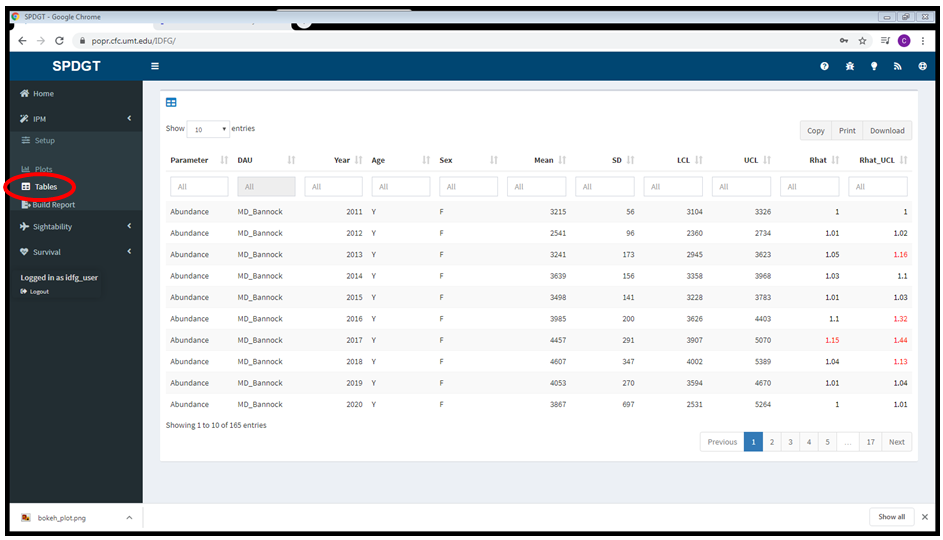
\includegraphics{./www/ipm_11.PNG}

\begin{enumerate}
\def\labelenumi{\arabic{enumi}.}
\setcounter{enumi}{11}
\tightlist
\item
  Now build a report to see more diagnostic information. Click \textbf{Build Report} in the sidebar, then click the download button.
\end{enumerate}

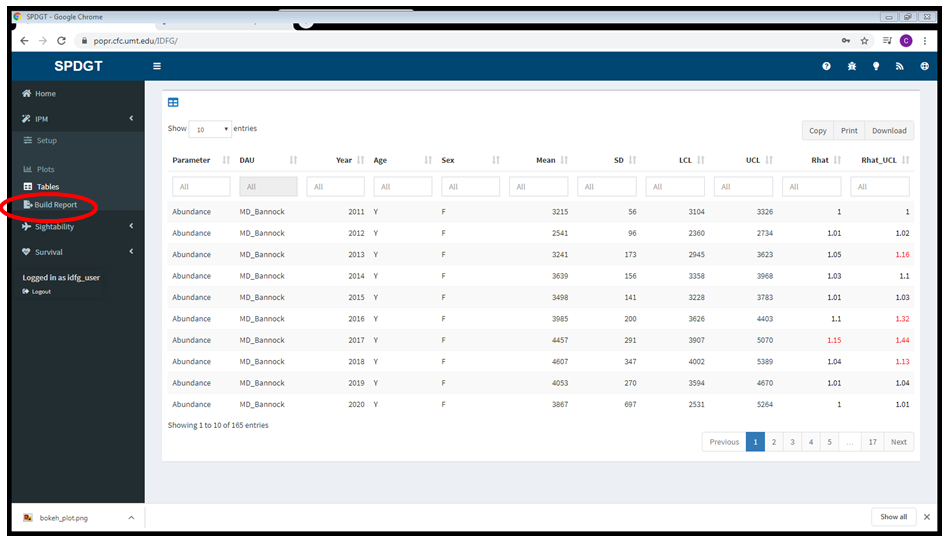
\includegraphics{./www/ipm_12.PNG}

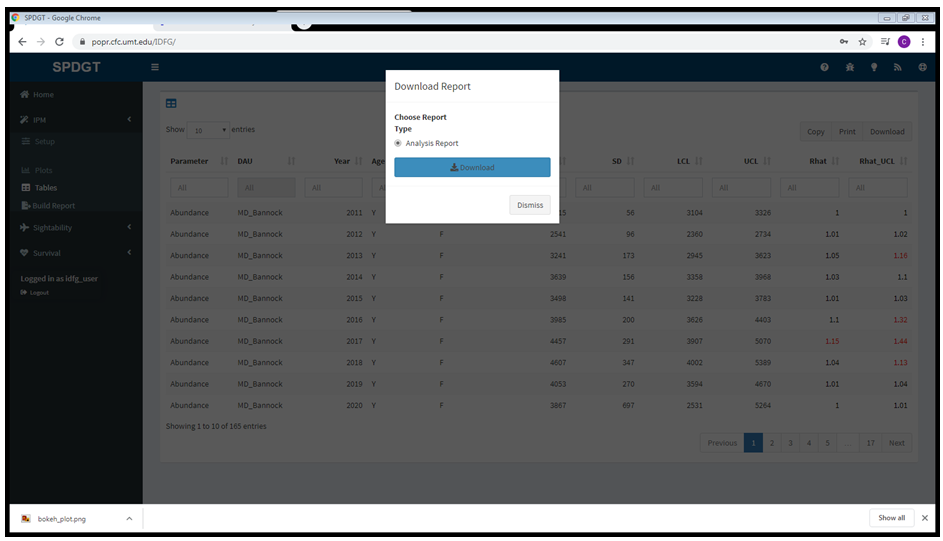
\includegraphics{./www/ipm_13.PNG}

\begin{enumerate}
\def\labelenumi{\arabic{enumi}.}
\setcounter{enumi}{12}
\tightlist
\item
  Notice the diagnostic section in red, indicating that the model did not converge. In some cases this may indicate problems with the data or the model structure, but sometimes we just need to let the model run longer.
\end{enumerate}

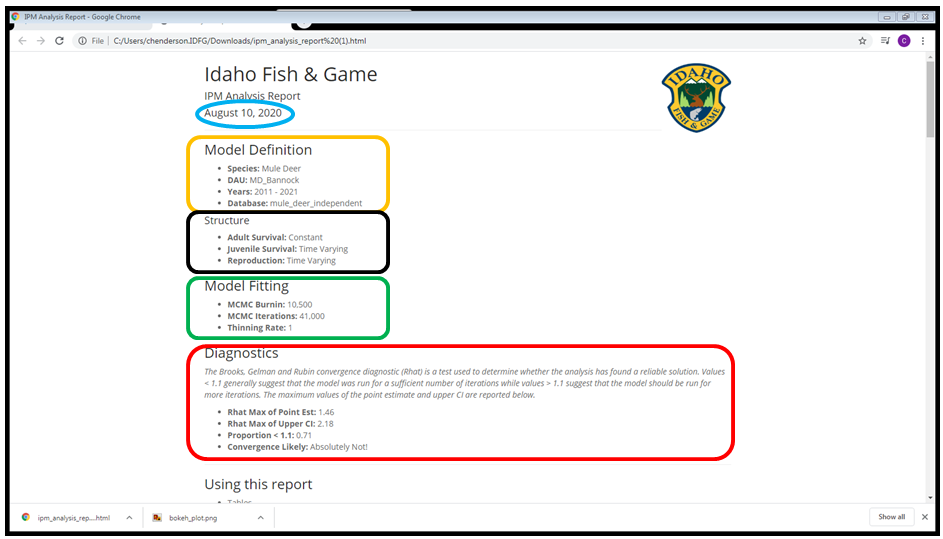
\includegraphics{./www/ipm_14.PNG}

\begin{enumerate}
\def\labelenumi{\arabic{enumi}.}
\setcounter{enumi}{13}
\tightlist
\item
  Return to the Run tab on the \textbf{setup} page and click the checkbox to \protect\hyperlink{gl-converge}{automate convergence}, then run the model again.
\end{enumerate}

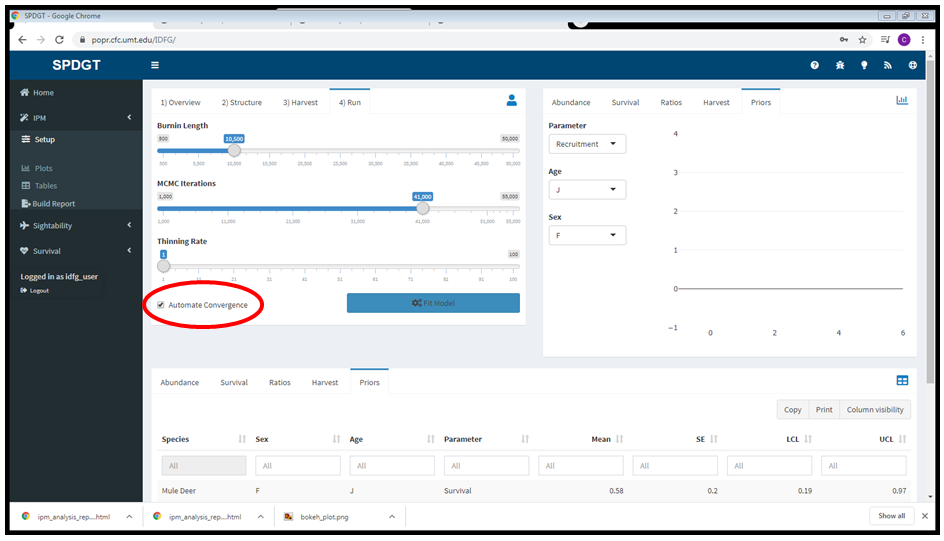
\includegraphics{./www/ipm_15.PNG}

\begin{enumerate}
\def\labelenumi{\arabic{enumi}.}
\setcounter{enumi}{14}
\tightlist
\item
  Build a new report and check the diagnostics section again. Allowing the model to run as long as needed resulted in much better performance.
\end{enumerate}

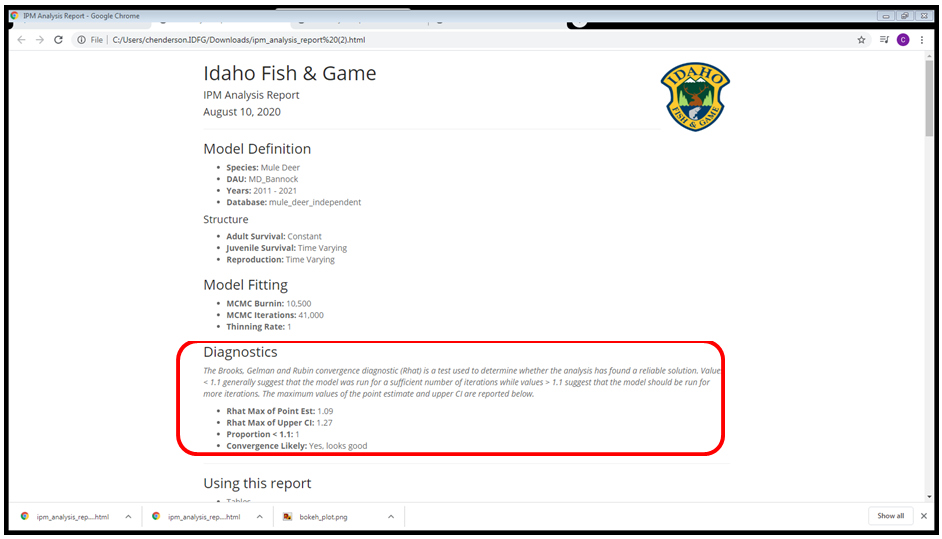
\includegraphics{./www/ipm_16.PNG}

\begin{enumerate}
\def\labelenumi{\arabic{enumi}.}
\setcounter{enumi}{15}
\tightlist
\item
  Check out the tables and plots in the rest of the report to review your results.
\end{enumerate}

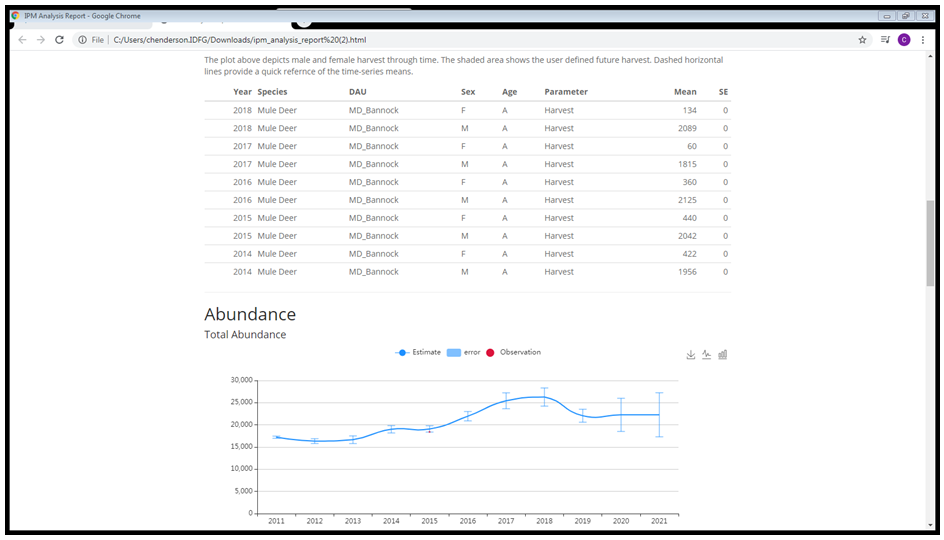
\includegraphics{./www/ipm_18.PNG}

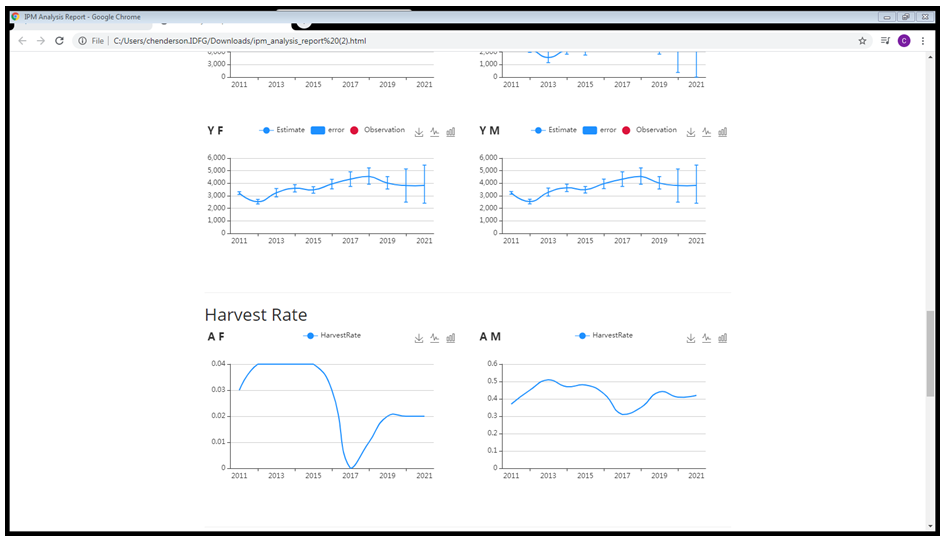
\includegraphics{./www/ipm_20.PNG}

\hypertarget{gl}{%
\chapter{Glossary}\label{gl}}

\hypertarget{gl-general}{%
\section{General}\label{gl-general}}

\hypertarget{gl-age-classes}{%
\subparagraph*{Age Classes}\label{gl-age-classes}}
\addcontentsline{toc}{subparagraph}{Age Classes}

Age classes must be defined for each species to capture variability in parameters like survival and harvest rate, as well as to determine when animals begin to reproduce. Regardless of actual birth date, animals transition to the next age class on December 15, the model anniversary used in the IPM. Assuming calves and fawns are born approximately mid-June each year, the age classes translate to roughly the following:

\begin{itemize}
\tightlist
\item
  Mule Deer

  \begin{itemize}
  \tightlist
  \item
    A (Adult) - 1.5 years and up
  \item
    J (Juvenile) - 6 months to 1.5years
  \item
    Y (Young of Year) - birth to 6 months
  \end{itemize}
\item
  Elk

  \begin{itemize}
  \tightlist
  \item
    A (Adult) - 2.5 years and up
  \item
    S (SubAdult) - 1.5 to 2.5 years
  \item
    J (Juvenile) - 6 months to 1.5 years
  \item
    Y (Young of Year) - birth to 6 months
  \end{itemize}
\end{itemize}

\hypertarget{gl-bio-year}{%
\subparagraph*{Bio Year}\label{gl-bio-year}}
\addcontentsline{toc}{subparagraph}{Bio Year}

Since winter surveys typically span a time period including two years the term BioYear consolidates the survey period into a single year. For example, surveys can start in December 2019 and run through January 2020 so the BioYear for this survey is 2020. The term was created for easier record keeping and does not have a biological definition. The biological year begins on December 15 and was intended to correctly align data collection with biological processes. Estimates from the models operate on this biological year.

\hypertarget{gl-dau}{%
\subparagraph*{DAU (Data Analysis Unit)}\label{gl-dau}}
\addcontentsline{toc}{subparagraph}{DAU (Data Analysis Unit)}

Recent location data from mule deer fitted with GPS radio-collars provided a more informed understanding of how mule deer populations are distributed across Idaho. In light of this new information, IDFG revised the geographical boundaries of the data analysis units (DAU) that are used for mule deer population monitoring and management and incorporated these changes into the IPM. Some aerial surveys can no longer be viewed in the IPM because they don't include abundance for all of the GMUs in the new DAU. Past aerial surveys were incorporated into the site through a series of conversations with area biologists. Questions about the data can be directed to Paul Atwood or Josh Nowak.

\hypertarget{gl-samm}{%
\subparagraph*{SAMM (AKA SAD)}\label{gl-samm}}
\addcontentsline{toc}{subparagraph}{SAMM (AKA SAD)}

SAMM, or Statewide Animal Monitoring Master, is a database hosted by IDFG for housing monitoring data. Data is read into PopR from SAMM via API, but SAMM data cannot be edited through PopR. In order to add or edit data the changes must be made in SAMM.

\hypertarget{gl-sight}{%
\section{Sightability}\label{gl-sight}}

\hypertarget{gl-aircraft}{%
\subparagraph*{Aircraft/Model}\label{gl-aircraft}}
\addcontentsline{toc}{subparagraph}{Aircraft/Model}

There are separate elk sightability models depending on the aircraft used for the survey. The aircraft types include a Hiller 12E, Bell 47G, and Super Cub. Mule deer sightability models do not have separate models for different types of aircraft.

\hypertarget{gl-area}{%
\subparagraph*{Area}\label{gl-area}}
\addcontentsline{toc}{subparagraph}{Area}

A generic term used to catch the species specific differences in management area naming. Instead of elk zones and deer pmu/dau we simply use area to describe the spatial extent we are focused on for a particular analysis.

\hypertarget{gl-comp-survey}{%
\subparagraph*{Composition Survey}\label{gl-comp-survey}}
\addcontentsline{toc}{subparagraph}{Composition Survey}

This survey type is used to gather data related to age and sex ratios and typically samples a smaller portion of the population in an area of interest. See also: \protect\hyperlink{gl-sight-survey}{Sightability Survey}

\hypertarget{gl-demographic}{%
\subparagraph*{Demographic}\label{gl-demographic}}
\addcontentsline{toc}{subparagraph}{Demographic}

The demographic field in the sightability output table denotes which age and sex classes are described by the estimated values. Classes are based on on sex and \protect\hyperlink{gl-age-classes}{age class} and vary by species and survey type.

\hypertarget{gl-group-size}{%
\subparagraph*{Group size}\label{gl-group-size}}
\addcontentsline{toc}{subparagraph}{Group size}

Refers to the number of individuals in a single observed group. The size of the group impacts the probability of detection and influences how the model estimates the true number of individuals. Group sizes include 1, 2, 3, 4, 5, 6, 7-15, 16-30, and \textgreater30.

\hypertarget{gl-movement}{%
\subparagraph*{Movement Categories}\label{gl-movement}}
\addcontentsline{toc}{subparagraph}{Movement Categories}

The 3 movement categories are bedded, standing, and moving. This is based on the most active individual when initially observed. The movement categories impact the probability of detection and influence how the model estimates the true number of individuals.

\hypertarget{gl-obs}{%
\subparagraph*{Obs}\label{gl-obs}}
\addcontentsline{toc}{subparagraph}{Obs}

The number of observations in a given strata.

\hypertarget{gl-pop}{%
\subparagraph*{Pop}\label{gl-pop}}
\addcontentsline{toc}{subparagraph}{Pop}

The population of sampling units in a given strata. In other words, the total number of subunits in a strata.

\hypertarget{gl-prop-sampled}{%
\subparagraph*{PropSampled}\label{gl-prop-sampled}}
\addcontentsline{toc}{subparagraph}{PropSampled}

This is the proportion of units sampled in a given strata. This can be calculated by obs/pop, divide the number of subunits sampled in the strata by the total number of subunits in the strata.

\hypertarget{gl-sight-survey}{%
\subparagraph*{Sightability Survey}\label{gl-sight-survey}}
\addcontentsline{toc}{subparagraph}{Sightability Survey}

An intensive aerial survey methodology to estimate the entire population size in a given area. Data, in the form of raw counts, from this survey are analyzed using a sightability model to estimate true population size from direct counts. See also: \protect\hyperlink{gl-comp-survey}{Composition Survey}

\hypertarget{gl-snow}{%
\subparagraph*{Snow}\label{gl-snow}}
\addcontentsline{toc}{subparagraph}{Snow}

The 3 snow cover categories are 0-20\%, 21-79\%, and \textgreater80\%. The snow cover categories impact the probability of detection and influences how the model estimates the true number of individuals.

\hypertarget{gl-stratum}{%
\subparagraph*{Stratum}\label{gl-stratum}}
\addcontentsline{toc}{subparagraph}{Stratum}

The landscape is divided into separate strata based on the probability of being occupied by the species being surveyed. Typically subunits are classified as high, medium, or low strata based on their suitability as habitat for a particular species. Other strata should only be used after consulting an expert and in special circumstances when you do not want that subunit to be used to extrapolate to subunits that are not flown.

\hypertarget{gl-subunit}{%
\subparagraph*{Subunit}\label{gl-subunit}}
\addcontentsline{toc}{subparagraph}{Subunit}

Used to define the proportion of the unit that was sampled.For example, if a unit consists of 10 subunits and the survey samples 3 of the 10 subunits then 3/10 or .3 of the unit was sampled. This is used to extrapolate sightability estimates such that if this same survey produced a count of 100 then the estimate is 100/.3 or 333 animals in the unit.

\hypertarget{gl-unit}{%
\subparagraph*{Unit}\label{gl-unit}}
\addcontentsline{toc}{subparagraph}{Unit}

Synonymous with GMU.

\hypertarget{gl-variance}{%
\subparagraph*{Variance}\label{gl-variance}}
\addcontentsline{toc}{subparagraph}{Variance}

The variance components of the sightability output are of interest to the user because they provide clues as to how to improve their surveys.

\begin{itemize}
\tightlist
\item
  ModelVar: Model variance
\item
  SampleVar: Sample variance
\item
  SightVar: Sightability model variance
\item
  TotalVar: Total variance is the sum of the model, sample,and sightability variances. The square root of the total variance is the standard deviation of the estimated value.
\end{itemize}

\hypertarget{gl-veg}{%
\subparagraph*{Vegetation}\label{gl-veg}}
\addcontentsline{toc}{subparagraph}{Vegetation}

There are 5 vegetation class categories including grass/open/agriculture, sagebrush, juniper/mtn. mahogany, mtn. brush/aspen, and conifer. Vegetation class represents the dominant vegetation within a 30m buffer around where an individual deer or group of deer is observed. The vegetation class categories impact the probability of detection and influences how the model estimates the true number of individuals. PopR has data columns for all habitat data collected on IDFG elk and mule deer sightability and composition survey forms. IDFG elk aerial survey data sheets contain only \% screen and that is the only habitat variable used in the elk sightability model. IDFG mule deer aerial survey and composition data sheets contain data columns for \% screen, screen type, and veg type and veg type is the only habitat variable currently used in the mule deer sightability model.

\hypertarget{gl-surv}{%
\section{Survival}\label{gl-surv}}

\hypertarget{gl-known-fate}{%
\subparagraph*{Known Fate Survival Model}\label{gl-known-fate}}
\addcontentsline{toc}{subparagraph}{Known Fate Survival Model}

Survival models attempt to estimate the probability that an animal alive at this time will be alive at some future time. A known-fate model does this in part by assuming that the fate of every animal is known. This name was chosen early in the development process. As time has passed we have tweaked and developed the model to relax assumptions and better meet the needs of our collaborators. The full model description is beyond the scope of this Glossary, but know that the Known-Fate model selection means that the results of running a model will show the user estimates of survival and mortality. This is in contrast to the multi-state models where multiple sources of mortality can be estimated, such as death by harvest or death by predator. See also: \protect\hyperlink{gl-multi-state}{Multi-state Survival Model}

\hypertarget{gl-multi-state}{%
\subparagraph*{Multi-state Survival Model}\label{gl-multi-state}}
\addcontentsline{toc}{subparagraph}{Multi-state Survival Model}

The multi-state survival model allows users to estimate survival, harvest mortality rate and other mortality rate. The different estimates sum to 1 and so to be comparable to the known-fate models users should take 1 - other mortality as equivalent to survival in the known-fate context. See also: \protect\hyperlink{gl-known-fate}{Known Fate Survival Model}

\hypertarget{gl-ipm}{%
\section{IPM}\label{gl-ipm}}

\hypertarget{gl-ipm-db}{%
\subparagraph*{IPM Database}\label{gl-ipm-db}}
\addcontentsline{toc}{subparagraph}{IPM Database}

IPM database files contain the estimates from survival and sightability models, and are used when running the IPM. As of September 2020 there are 3 IPM database files in use for IDFG:

\begin{enumerate}
\def\labelenumi{\arabic{enumi}.}
\tightlist
\item
  Atwood.RData -- DO NOT USE, this database is for development and research purposes only
\item
  mule\_deer\_independent.RData -- This database will use survival data from the DAU you are modeling over multiple years when there is not any survival data for the DAU and the year in the database. Use this database if the DAU you are modeling has a large amount of data available and survival is relatively constant between years.
\item
  mule\_deer\_shared.RData - Strongly recommended. This database will use survival data from other DAU's in the state for the current year when there is not any survival data for the DAU and year in the database. Use this database if the DAU you are modeling has little to no data available or if survival is highly variable between years.
\end{enumerate}

\hypertarget{gl-ipm-weather}{%
\subparagraph*{Future Weather}\label{gl-ipm-weather}}
\addcontentsline{toc}{subparagraph}{Future Weather}

Future weather covariates were developed using Mark Hurley's dissertation and the analyses contained therein.

\begin{itemize}
\tightlist
\item
  Average: Mean observed weather conditions
\item
  Good: Upper 95\% quantile of observed weather
\item
  Bad: Lower 5\% quantile of observed weather
\item
  None: Do not use weather data covariates in the analysis
\end{itemize}

\hypertarget{gl-mcmc}{%
\section{MCMC}\label{gl-mcmc}}

\hypertarget{gl-converge}{%
\subparagraph*{Automate Convergence}\label{gl-converge}}
\addcontentsline{toc}{subparagraph}{Automate Convergence}

Users may choose to simply check the ``Automate Convergence'' box below the MCMC sliders menu in the PopR interface. This option will assure that an adequate Burn-in Length and number of MCMC Iterations have been used to produce a statistically sound estimate and error distribution.

\hypertarget{gl-burn-in}{%
\subparagraph*{Burnin Length}\label{gl-burn-in}}
\addcontentsline{toc}{subparagraph}{Burnin Length}

``Burn-in'' is a term for an initial process that gives the Markov Chain time to approach the solution to the problem by throwing away some less reasonable starting points at the beginning of a Markov Chain Monte Carlo run. In PopR, managers should simply use the default Burn-in Length setting when developing an estimate through the standard user interface.

\hypertarget{gl-iter}{%
\subparagraph*{Iterations}\label{gl-iter}}
\addcontentsline{toc}{subparagraph}{Iterations}

PopR uses Markov Chain Monte Carlo (MCMC) methods to ``fit'' IPM population estimates to the available data. MCMC methods estimate parameters in complex models by systematically updating informed prior distributions with information gleaned from field data (e.g.~observed harvest). Therefore, they allow us to describe each parameter in terms of a distribution and that distribution's shape. Typically, 25,000-100,000 MCMC iterations will be required to fit an IPM. If the number of MCMC iterations is set too low the uncertainty about an estimate is likely to be misrepresented.

\hypertarget{gl-rhat}{%
\subparagraph*{Brooks-Gelman-Rubin Statistic (R̂)}\label{gl-rhat}}
\addcontentsline{toc}{subparagraph}{Brooks-Gelman-Rubin Statistic (R̂)}

In PopR, we use the Brooks-Gelman-Rubin (BGR) statistic, often represented as R̂ or Rhat, as an assessment of convergence and the criteria used when the ``Automate Convergence'' option is used. The BGR statistic suggests convergence when estimates of R̂ are below 1.1 or more generally close to 1. This statistic is reported in the output tables for most models and highlighted in red when R̂ estimates are above 1.1. The default settings will produce results that are unlikely to change even if run longer, but users should increase the number of MCMC iterations if R̂ estimates are above 1.1 and computing time allows.

\hypertarget{gl-thin}{%
\subparagraph*{Thinning Rate}\label{gl-thin}}
\addcontentsline{toc}{subparagraph}{Thinning Rate}

Thinning tells the sampler to only retain every nth value from the chains. This technique is sometimes used to reduce autocorrelation in the chains, but comes at the cost of reduced efficiency of the sampler. A more reasonable use of thinning is when hardware limitations are being reached, which typically comes in the form of running out of memory. This will not be an issue in PopR and, therefore, the recommended setting for the Thinning slider is 1.

\end{document}
